\hypertarget{group__geometry}{
\section{Geometria}
\label{group__geometry}\index{Geometria@{Geometria}}
}


\subsection{Descripci\'{o}n detallada}
Son los modelos y estructuras geometricas utilizadas para calcular las caracteristicas del problema, debido a que nesting esta fuertemente enlazado con poligonos, es necesario implementar el conjunto de objetos geometricos que lo manejen. 

\subsection*{Archivos}
\begin{CompactItemize}
\item 
archivo \hyperlink{line_8h}{line.h}
\item 
archivo \hyperlink{point_8h}{point.h}
\item 
archivo \hyperlink{polygon_8h}{polygon.h}
\item 
archivo \hyperlink{polygon__holes_8h}{polygon\_\-holes.h}
\item 
archivo \hyperlink{line_8c}{line.c}
\item 
archivo \hyperlink{point_8c}{point.c}
\item 
archivo \hyperlink{polygon_8c}{polygon.c}
\item 
archivo \hyperlink{polygon__holes_8c}{polygon\_\-holes.c}
\end{CompactItemize}
\subsection*{Clases}
\begin{CompactItemize}
\item 
struct \hyperlink{struct__line}{\_\-line}
\item 
struct \hyperlink{struct__point}{\_\-point}
\item 
struct \hyperlink{struct__polygon}{\_\-polygon}
\item 
struct \hyperlink{struct__polygon__holes}{\_\-polygon\_\-holes}
\end{CompactItemize}
\subsection*{Tipos definidos}
\begin{CompactItemize}
\item 
typedef \hyperlink{struct__line}{\_\-line} \hyperlink{group__geometry_gbb4d6a1464226fe9b7c0d80348e5eb98_gbb4d6a1464226fe9b7c0d80348e5eb98}{line}
\item 
typedef \hyperlink{struct__point}{\_\-point} \hyperlink{group__geometry_g37e9de632d1eb76ff7dcd3d8172add7d_g37e9de632d1eb76ff7dcd3d8172add7d}{point}
\item 
typedef \hyperlink{struct__polygon}{\_\-polygon} \hyperlink{group__geometry_g9169f21a34d344b356c44948943e99cc_g9169f21a34d344b356c44948943e99cc}{polygon}
\item 
typedef \hyperlink{struct__polygon__holes}{\_\-polygon\_\-holes} \hyperlink{group__geometry_g1137695e6ed0a9b25685f8bf3ccdb45f_g1137695e6ed0a9b25685f8bf3ccdb45f}{polygon\_\-holes}
\end{CompactItemize}
\subsection*{Funciones}
\begin{CompactItemize}
\item 
bool \hyperlink{group__geometry_g95f804c79e71c1ca62453b6f0123e307_g95f804c79e71c1ca62453b6f0123e307}{line\_\-intersection} (\hyperlink{struct__line}{line} $\ast$l1, \hyperlink{struct__line}{line} $\ast$l2)
\item 
bool \hyperlink{group__geometry_ga27fbafb04a36a60af7bd5cafbdfd412_ga27fbafb04a36a60af7bd5cafbdfd412}{line\_\-equal} (\hyperlink{struct__line}{line} $\ast$l1, \hyperlink{struct__line}{line} $\ast$l2)
\item 
bool \hyperlink{group__geometry_g68d4dad9b8e742b0d63affc853f80391_g68d4dad9b8e742b0d63affc853f80391}{line\_\-ispoint} (\hyperlink{struct__line}{line} $\ast$l1)
\item 
float \hyperlink{group__geometry_ga7ae8d919209fea43e8a61215398bbbe_ga7ae8d919209fea43e8a61215398bbbe}{point\_\-dot} (\hyperlink{struct__point}{point} $\ast$a, \hyperlink{struct__point}{point} $\ast$b, \hyperlink{struct__point}{point} $\ast$c)
\item 
float \hyperlink{group__geometry_gb97527165a510655ee37cd3ccfa8d932_gb97527165a510655ee37cd3ccfa8d932}{point\_\-cross} (\hyperlink{struct__point}{point} $\ast$a, \hyperlink{struct__point}{point} $\ast$b, \hyperlink{struct__point}{point} $\ast$c)
\item 
float \hyperlink{group__geometry_gcfbc9e7772d80361768bc0b65cebbca1_gcfbc9e7772d80361768bc0b65cebbca1}{polygon\_\-area} (\hyperlink{struct__polygon}{polygon} $\ast$p)
\item 
bool \hyperlink{group__geometry_geab0a1d6da7c44ae49494958bb885504_geab0a1d6da7c44ae49494958bb885504}{polygon\_\-pointin} (\hyperlink{struct__polygon}{polygon} $\ast$p, \hyperlink{struct__point}{point} $\ast$f)
\item 
bool \hyperlink{group__geometry_g2be6101a257ea8896e61e93d14b22b89_g2be6101a257ea8896e61e93d14b22b89}{polygon\_\-overlapping} (\hyperlink{struct__polygon}{polygon} $\ast$p, \hyperlink{struct__polygon}{polygon} $\ast$q)
\item 
void \hyperlink{group__geometry_g95276abee7240f116afaf80a3e1f23c4_g95276abee7240f116afaf80a3e1f23c4}{polygon\_\-rotate} (\hyperlink{struct__polygon}{polygon} $\ast$p, float t)
\item 
void \hyperlink{group__geometry_g137ef6f552a0a04c5ae0493690088f3f_g137ef6f552a0a04c5ae0493690088f3f}{polygon\_\-minbox} (\hyperlink{struct__polygon}{polygon} $\ast$p, float $\ast$minx, float $\ast$miny, float $\ast$maxx, float $\ast$maxy)
\item 
void \hyperlink{group__geometry_g7538c2bf0d1e8acc0cfc055b6bf3a96b_g7538c2bf0d1e8acc0cfc055b6bf3a96b}{polygon\_\-translate} (\hyperlink{struct__polygon}{polygon} $\ast$p, float x, float y)
\item 
float \hyperlink{group__geometry_g380cdcfa6caf51828c8d06f4518a4084_g380cdcfa6caf51828c8d06f4518a4084}{polygonholes\_\-area} (\hyperlink{struct__polygon__holes}{polygon\_\-holes} $\ast$p)
\item 
float \hyperlink{group__geometry_g7cf8b3f8c76179bb936754bbbf510999_g7cf8b3f8c76179bb936754bbbf510999}{polygonholes\_\-volumen} (\hyperlink{struct__polygon__holes}{polygon\_\-holes} $\ast$p)
\item 
bool \hyperlink{group__geometry_g35a6dd45f6d0cbed26ef8a69ed34a2e9_g35a6dd45f6d0cbed26ef8a69ed34a2e9}{polygonholes\_\-pointin} (\hyperlink{struct__polygon__holes}{polygon\_\-holes} $\ast$p, \hyperlink{struct__point}{point} $\ast$f)
\item 
bool \hyperlink{group__geometry_g496bae87588cb5710ced80f713da98ad_g496bae87588cb5710ced80f713da98ad}{polygonholes\_\-polygonin} (\hyperlink{struct__polygon__holes}{polygon\_\-holes} $\ast$p, \hyperlink{struct__polygon}{polygon} $\ast$q)
\item 
bool \hyperlink{group__geometry_g139317720b027c782db9424256ba2c2d_g139317720b027c782db9424256ba2c2d}{polygonholes\_\-pointinhole} (\hyperlink{struct__polygon__holes}{polygon\_\-holes} $\ast$p, \hyperlink{struct__point}{point} $\ast$f)
\item 
\hyperlink{struct__point}{point} \hyperlink{group__geometry_ge39fef354e4411678ec081c197b29825_ge39fef354e4411678ec081c197b29825}{polygon\_\-center} (\hyperlink{struct__polygon}{polygon} $\ast$p)
\end{CompactItemize}


\subsection{Documentaci\'{o}n de los tipos definidos}
\hypertarget{group__geometry_gbb4d6a1464226fe9b7c0d80348e5eb98_gbb4d6a1464226fe9b7c0d80348e5eb98}{
\index{geometry@{geometry}!line@{line}}
\index{line@{line}!geometry@{geometry}}
\subsubsection[line]{\setlength{\rightskip}{0pt plus 5cm}typedef struct \hyperlink{struct__line}{\_\-line} \hyperlink{struct__line}{line}}}
\label{group__geometry_gbb4d6a1464226fe9b7c0d80348e5eb98_gbb4d6a1464226fe9b7c0d80348e5eb98}




Definici\'{o}n en la l\'{\i}nea 21 del archivo line.h.\hypertarget{group__geometry_g37e9de632d1eb76ff7dcd3d8172add7d_g37e9de632d1eb76ff7dcd3d8172add7d}{
\index{geometry@{geometry}!point@{point}}
\index{point@{point}!geometry@{geometry}}
\subsubsection[point]{\setlength{\rightskip}{0pt plus 5cm}typedef struct \hyperlink{struct__point}{\_\-point} \hyperlink{struct__point}{point}}}
\label{group__geometry_g37e9de632d1eb76ff7dcd3d8172add7d_g37e9de632d1eb76ff7dcd3d8172add7d}




Definici\'{o}n en la l\'{\i}nea 17 del archivo point.h.\hypertarget{group__geometry_g9169f21a34d344b356c44948943e99cc_g9169f21a34d344b356c44948943e99cc}{
\index{geometry@{geometry}!polygon@{polygon}}
\index{polygon@{polygon}!geometry@{geometry}}
\subsubsection[polygon]{\setlength{\rightskip}{0pt plus 5cm}typedef struct \hyperlink{struct__polygon}{\_\-polygon} \hyperlink{struct__polygon}{polygon}}}
\label{group__geometry_g9169f21a34d344b356c44948943e99cc_g9169f21a34d344b356c44948943e99cc}




Definici\'{o}n en la l\'{\i}nea 24 del archivo polygon.h.\hypertarget{group__geometry_g1137695e6ed0a9b25685f8bf3ccdb45f_g1137695e6ed0a9b25685f8bf3ccdb45f}{
\index{geometry@{geometry}!polygon_holes@{polygon\_\-holes}}
\index{polygon_holes@{polygon\_\-holes}!geometry@{geometry}}
\subsubsection[polygon\_\-holes]{\setlength{\rightskip}{0pt plus 5cm}typedef struct \hyperlink{struct__polygon__holes}{\_\-polygon\_\-holes} \hyperlink{struct__polygon__holes}{polygon\_\-holes}}}
\label{group__geometry_g1137695e6ed0a9b25685f8bf3ccdb45f_g1137695e6ed0a9b25685f8bf3ccdb45f}




Definici\'{o}n en la l\'{\i}nea 24 del archivo polygon\_\-holes.h.

\subsection{Documentaci\'{o}n de las funciones}
\hypertarget{group__geometry_ga27fbafb04a36a60af7bd5cafbdfd412_ga27fbafb04a36a60af7bd5cafbdfd412}{
\index{geometry@{geometry}!line_equal@{line\_\-equal}}
\index{line_equal@{line\_\-equal}!geometry@{geometry}}
\subsubsection[line\_\-equal]{\setlength{\rightskip}{0pt plus 5cm}bool line\_\-equal (\hyperlink{struct__line}{line} $\ast$ {\em l1}, \hyperlink{struct__line}{line} $\ast$ {\em l2})}}
\label{group__geometry_ga27fbafb04a36a60af7bd5cafbdfd412_ga27fbafb04a36a60af7bd5cafbdfd412}


Compara dos segmentos de linea, en este caso el orden de los extremos importa en la operacion

\begin{Desc}
\item[Par\'{a}metros:]
\begin{description}
\item[\mbox{$\leftarrow$} {\em l1}]Linea en 2 dimensiones \item[\mbox{$\leftarrow$} {\em l2}]Linea en 2 dimensiones \end{description}
\end{Desc}
\begin{Desc}
\item[Devuelve:]Verdadero si los segmentos de recta son iguales, falso en caso contrario \end{Desc}


Definici\'{o}n en la l\'{\i}nea 109 del archivo line.c.

\begin{Code}\begin{verbatim}110 {
111     return (l1->v1.x == l2->v1.x &&
112             l1->v1.y == l2->v1.y &&
113             l1->v2.x == l2->v2.x &&
114             l1->v2.y == l2->v2.y
115            ) ? true : false;
116 }
\end{verbatim}\end{Code}




Here is the caller graph for this function:\begin{figure}[H]
\begin{center}
\leavevmode
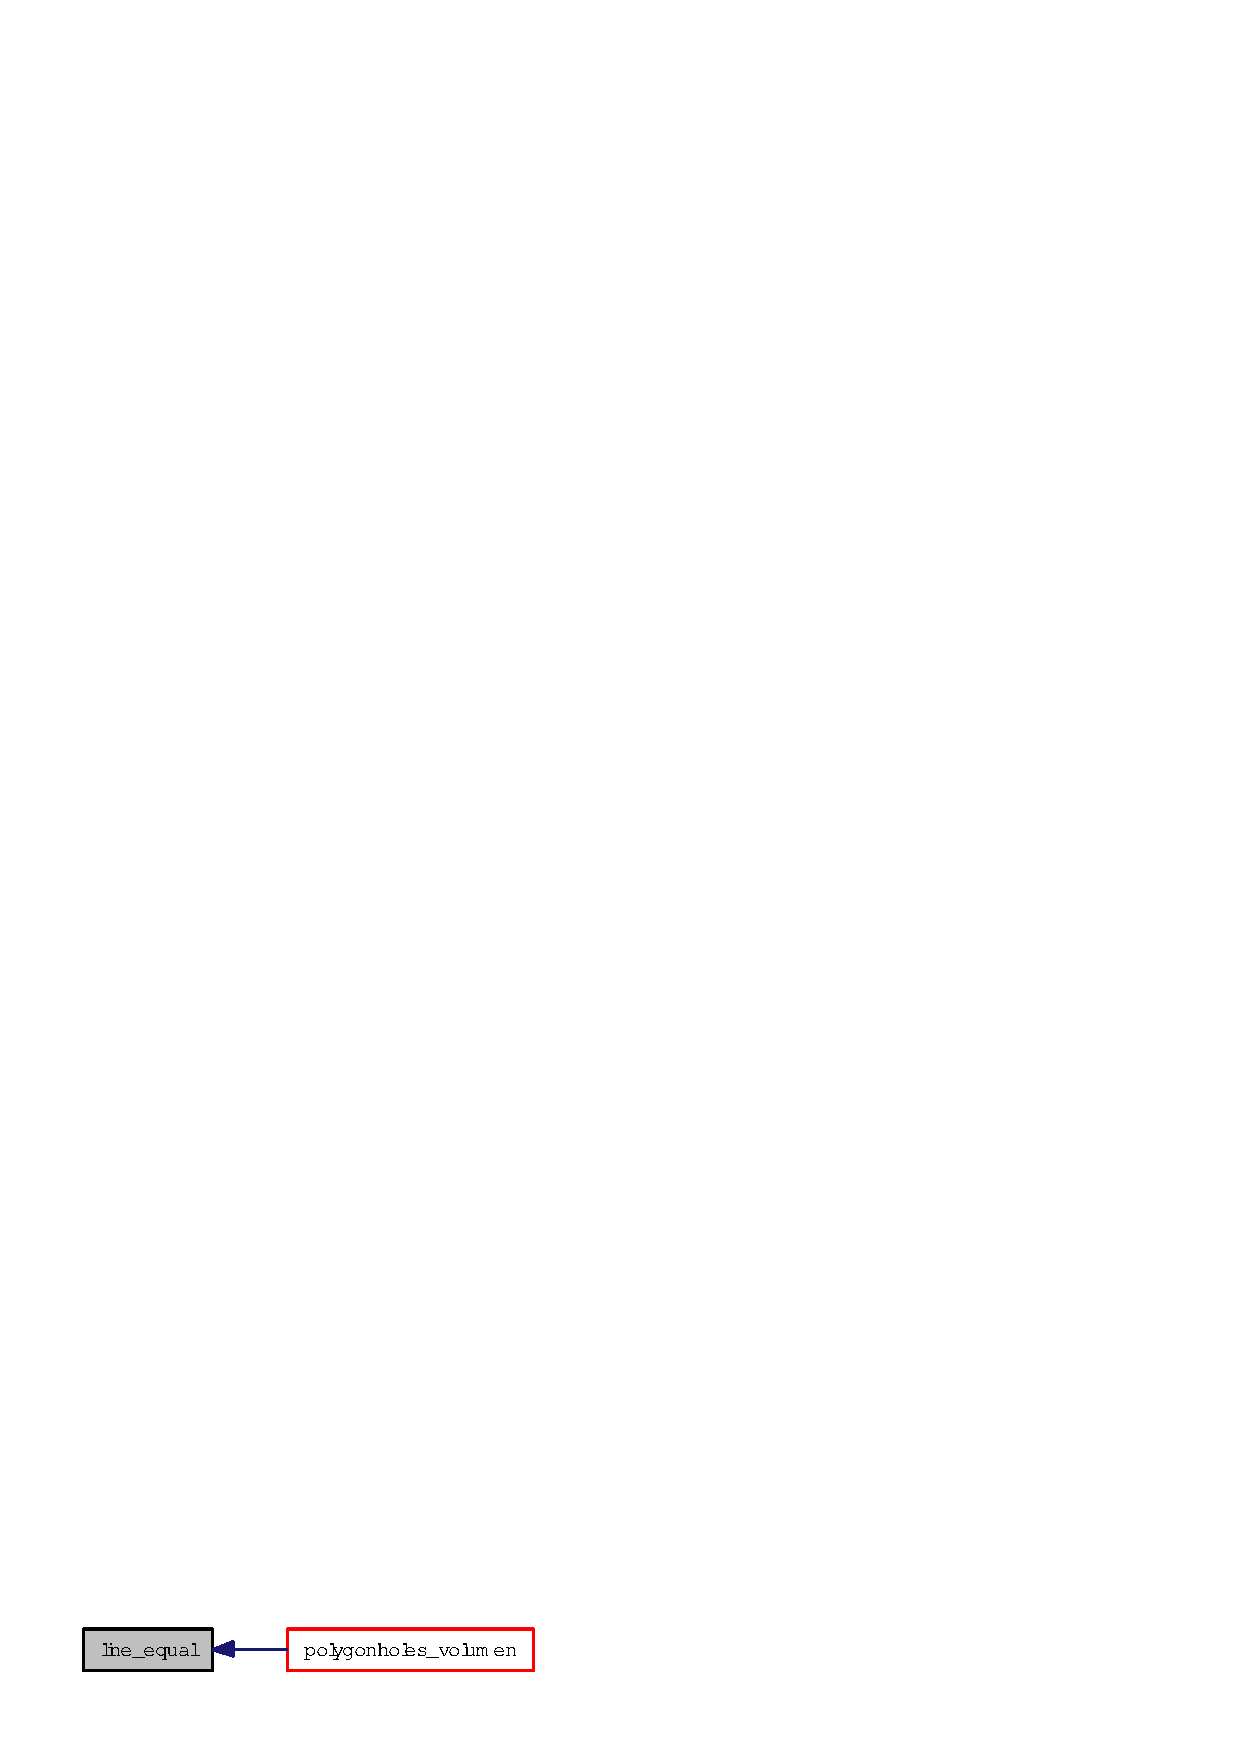
\includegraphics[width=130pt]{group__geometry_ga27fbafb04a36a60af7bd5cafbdfd412_ga27fbafb04a36a60af7bd5cafbdfd412_icgraph}
\end{center}
\end{figure}
\hypertarget{group__geometry_g95f804c79e71c1ca62453b6f0123e307_g95f804c79e71c1ca62453b6f0123e307}{
\index{geometry@{geometry}!line_intersection@{line\_\-intersection}}
\index{line_intersection@{line\_\-intersection}!geometry@{geometry}}
\subsubsection[line\_\-intersection]{\setlength{\rightskip}{0pt plus 5cm}bool line\_\-intersection (\hyperlink{struct__line}{line} $\ast$ {\em l1}, \hyperlink{struct__line}{line} $\ast$ {\em l2})}}
\label{group__geometry_g95f804c79e71c1ca62453b6f0123e307_g95f804c79e71c1ca62453b6f0123e307}


Identifica si dos lineas se intersectan, el algoritmo utilizado fue sacado del libro de Graphics Gems del Articulo Faster Line Segment Intersection

\begin{Desc}
\item[Par\'{a}metros:]
\begin{description}
\item[\mbox{$\leftarrow$} {\em l1}]Linea en 2 dimensiones \item[\mbox{$\leftarrow$} {\em l2}]Linea en 2 dimensiones \end{description}
\end{Desc}
\begin{Desc}
\item[Devuelve:]Un valor booleano que es verdadero si las lineas se intersectan y falso en caso contrario \end{Desc}


Definici\'{o}n en la l\'{\i}nea 22 del archivo line.c.

\begin{Code}\begin{verbatim}23 {
24     float x1,y1,x2,y2,x3,y3,x4,y4;
25     float Ax,Bx,Cx,Ay,By,Cy;
26     float x1lo,x1hi,y1lo,y1hi;
27     float d,e,f;
28 
29     x1 = l1->v1.x;
30     y1 = l1->v1.y;
31 
32     x2 = l1->v2.x;
33     y2 = l1->v2.y;
34 
35     x3 = l2->v1.x;
36     y3 = l2->v1.y;
37 
38     x4 = l2->v2.x;
39     y4 = l2->v2.y;
40 
41     Ax = x2 - x1;
42     Bx = x3 - x4;
43 
44     if (Ax < 0){
45         x1lo=x2;
46         x1hi=x1;
47     } else {
48         x1hi=x2;
49         x1lo=x1;
50     }
51 
52     if (Bx > 0){
53             if (x1hi < x4 || x2 < x1lo) return false;
54     } else {
55             if (x1hi < x3 || x4 < x1lo) return false;
56     }
57 
58     Ay = y2 - y1;
59     By = y3 - y4;
60 
61     if (Ay < 0){
62             y1lo = y2;
63             y1hi = y1;
64     } else {
65             y1hi = y2;
66             y1lo = y1;
67     }
68 
69     if (By > 0){
70             if (y1hi < y4 || y3 < y1lo) return false;
71     } else {
72             if (y1hi < y3 || y4 < y1lo) return false;
73     }
74 
75     Cx = x1 - x3;
76     Cy = y1 - y3;
77 
78     d = By*Cx - Bx*Cy;
79     f = Ay*Bx - Ax*By;
80 
81     if (f>0){
82             if (d<0 || d>f) return false;
83     } else {
84             if (d>0 || d<f) return false;
85     }
86 
87     e = Ax*Cy - Ay*Cx;
88 
89     if (f>0){
90             if (e<0 || e>f) return false;
91     } else {
92             if (e>0 || e<f) return false;
93     }
94 
95     if (f==0) return false;
96 
97     return true;
98 }
\end{verbatim}\end{Code}




Here is the caller graph for this function:\begin{figure}[H]
\begin{center}
\leavevmode
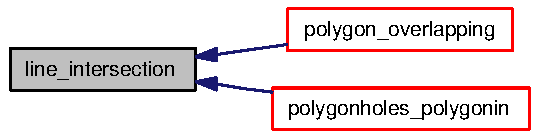
\includegraphics[width=147pt]{group__geometry_g95f804c79e71c1ca62453b6f0123e307_g95f804c79e71c1ca62453b6f0123e307_icgraph}
\end{center}
\end{figure}
\hypertarget{group__geometry_g68d4dad9b8e742b0d63affc853f80391_g68d4dad9b8e742b0d63affc853f80391}{
\index{geometry@{geometry}!line_ispoint@{line\_\-ispoint}}
\index{line_ispoint@{line\_\-ispoint}!geometry@{geometry}}
\subsubsection[line\_\-ispoint]{\setlength{\rightskip}{0pt plus 5cm}bool line\_\-ispoint (\hyperlink{struct__line}{line} $\ast$ {\em l})}}
\label{group__geometry_g68d4dad9b8e742b0d63affc853f80391_g68d4dad9b8e742b0d63affc853f80391}


Identifica si un segmento de recta es en realidad un unico punto, esto lo hace comprobando los puntos extremos del segmento de recta, si los extremos son iguales entonces se puede definir este segmento de recta como una linea

\begin{Desc}
\item[Par\'{a}metros:]
\begin{description}
\item[\mbox{$\leftarrow$} {\em l}]Linea en 2 dimensiones \end{description}
\end{Desc}
\begin{Desc}
\item[Devuelve:]Verdadero si la linea es un punto, falso en caso contrario. \end{Desc}


Definici\'{o}n en la l\'{\i}nea 128 del archivo line.c.

\begin{Code}\begin{verbatim}129 {
130     return (l->v1.x == l->v2.x && l->v1.y == l->v2.y) ? true : false;
131 }
\end{verbatim}\end{Code}




Here is the caller graph for this function:\begin{figure}[H]
\begin{center}
\leavevmode
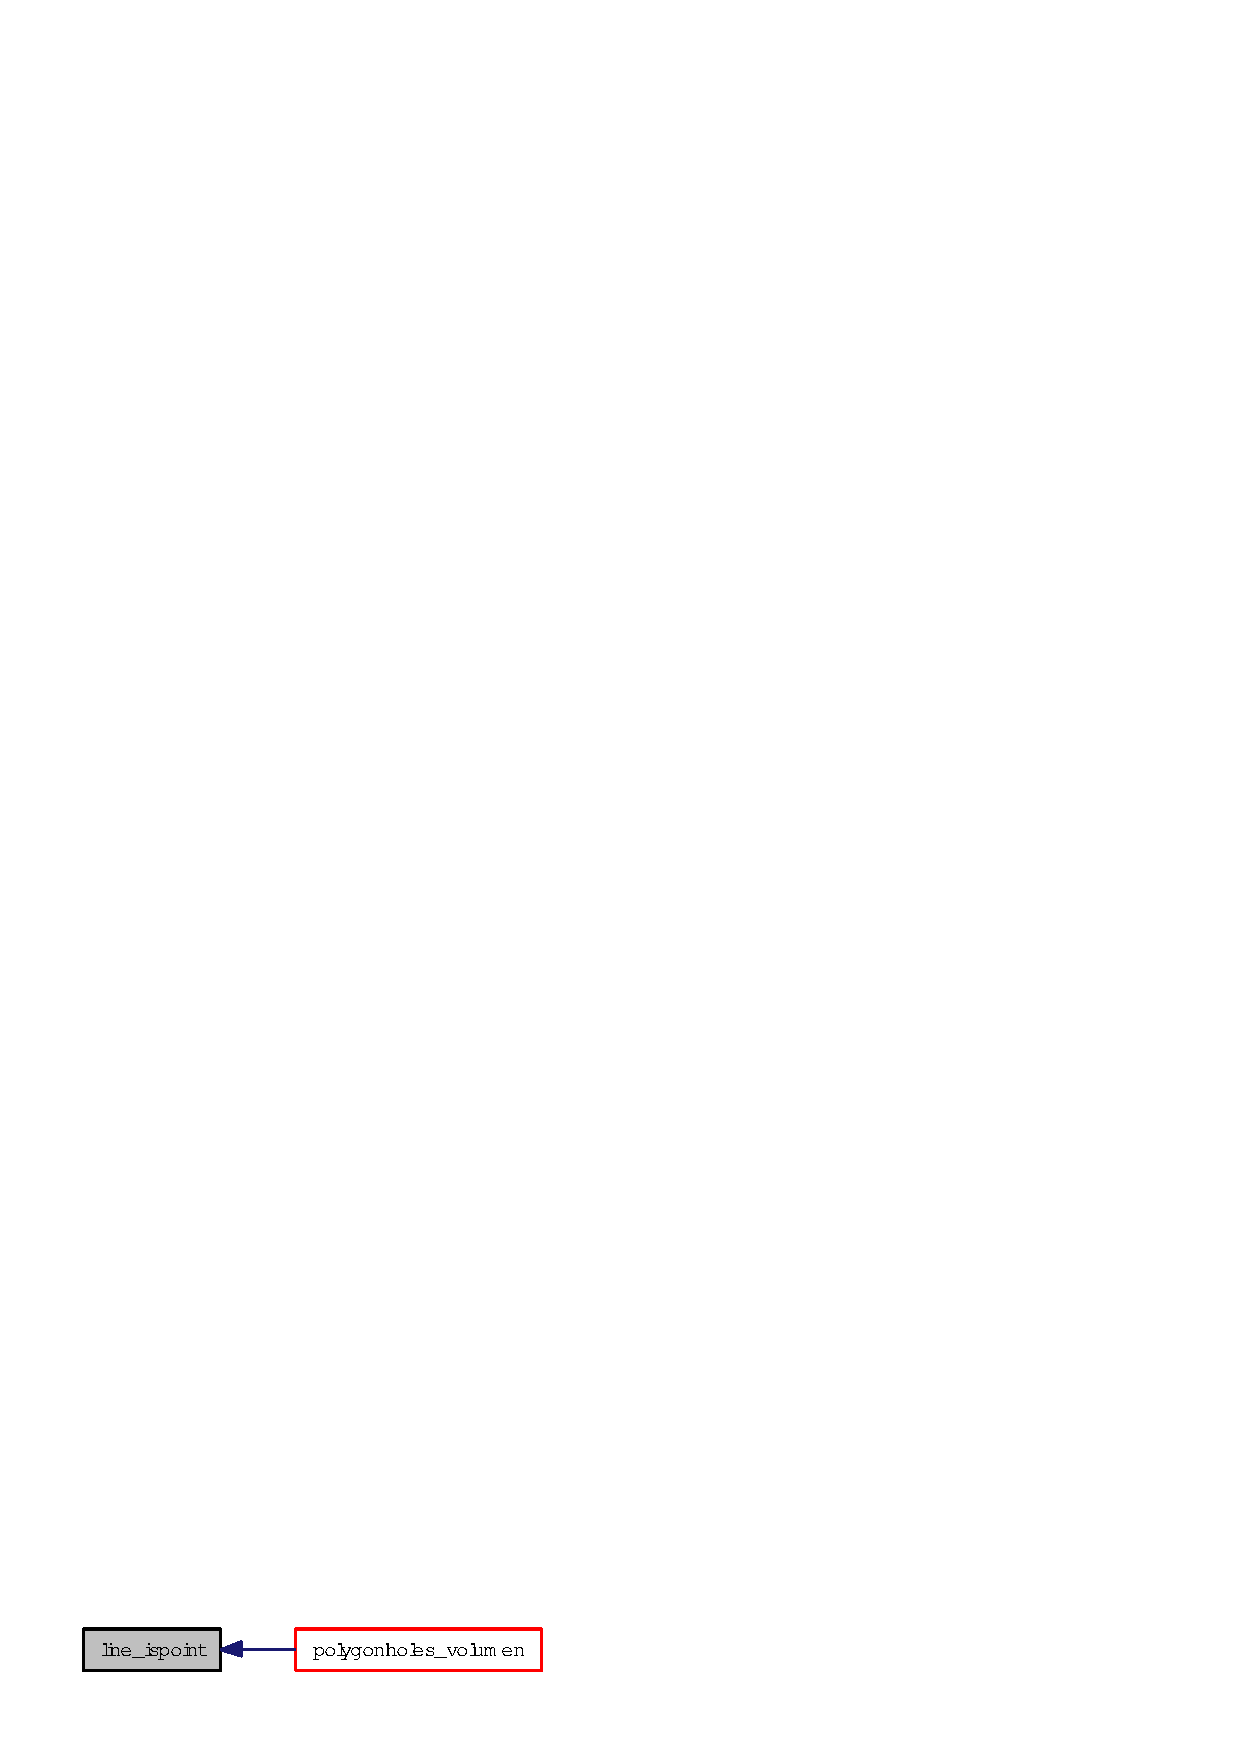
\includegraphics[width=132pt]{group__geometry_g68d4dad9b8e742b0d63affc853f80391_g68d4dad9b8e742b0d63affc853f80391_icgraph}
\end{center}
\end{figure}
\hypertarget{group__geometry_gb97527165a510655ee37cd3ccfa8d932_gb97527165a510655ee37cd3ccfa8d932}{
\index{geometry@{geometry}!point_cross@{point\_\-cross}}
\index{point_cross@{point\_\-cross}!geometry@{geometry}}
\subsubsection[point\_\-cross]{\setlength{\rightskip}{0pt plus 5cm}float point\_\-cross (\hyperlink{struct__point}{point} $\ast$ {\em a}, \hyperlink{struct__point}{point} $\ast$ {\em b}, \hyperlink{struct__point}{point} $\ast$ {\em c})}}
\label{group__geometry_gb97527165a510655ee37cd3ccfa8d932_gb97527165a510655ee37cd3ccfa8d932}


Calcula el producto cruz entro los punto a, b y c. Aunque esta funcion matematicamente esta definida en los vectores y no en los puntos, podemos relacionar un punto como el vector que hay desde el origen del plano hasta las coordenadas de este y asi calculamos el producto cruz.

\begin{Desc}
\item[Par\'{a}metros:]
\begin{description}
\item[\mbox{$\leftarrow$} {\em a}]Punto en 2 dimensiones \item[\mbox{$\leftarrow$} {\em b}]Punto en 2 dimensiones \item[\mbox{$\leftarrow$} {\em c}]Punto en 2 dimensiones \end{description}
\end{Desc}
\begin{Desc}
\item[Devuelve:]El producto cruz \end{Desc}


Definici\'{o}n en la l\'{\i}nea 38 del archivo point.c.

\begin{Code}\begin{verbatim}39 {
40     return ((b->x - a->x)*(c->y - a->y)) - ((b->y - a->y)*(c->x - a->x));
41 }
\end{verbatim}\end{Code}




Here is the caller graph for this function:\begin{figure}[H]
\begin{center}
\leavevmode
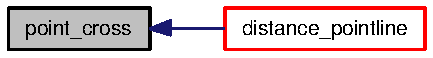
\includegraphics[width=122pt]{group__geometry_gb97527165a510655ee37cd3ccfa8d932_gb97527165a510655ee37cd3ccfa8d932_icgraph}
\end{center}
\end{figure}
\hypertarget{group__geometry_ga7ae8d919209fea43e8a61215398bbbe_ga7ae8d919209fea43e8a61215398bbbe}{
\index{geometry@{geometry}!point_dot@{point\_\-dot}}
\index{point_dot@{point\_\-dot}!geometry@{geometry}}
\subsubsection[point\_\-dot]{\setlength{\rightskip}{0pt plus 5cm}float point\_\-dot (\hyperlink{struct__point}{point} $\ast$ {\em a}, \hyperlink{struct__point}{point} $\ast$ {\em b}, \hyperlink{struct__point}{point} $\ast$ {\em c})}}
\label{group__geometry_ga7ae8d919209fea43e8a61215398bbbe_ga7ae8d919209fea43e8a61215398bbbe}


Calcula el producto punto entre los puntos a, b y c. Aunque esta funcion matematicamente esta definida en los vectores y no en los puntos, podemos relacionar un punto como el vector que hay desde el origen del plano hasta las coordenadas de este y asi calculamos el producto punto.

\begin{Desc}
\item[Par\'{a}metros:]
\begin{description}
\item[\mbox{$\leftarrow$} {\em a}]Punto en 2 dimensiones \item[\mbox{$\leftarrow$} {\em b}]Punto en 2 dimensiones \item[\mbox{$\leftarrow$} {\em c}]Punto en 2 dimensiones \end{description}
\end{Desc}
\begin{Desc}
\item[Devuelve:]El producto punto \end{Desc}


Definici\'{o}n en la l\'{\i}nea 21 del archivo point.c.

\begin{Code}\begin{verbatim}22 {
23     return ((b->x - a->x) * (c->x - b->x)) + ((b->y - a->y) * (c->y - b->y));
24 }
\end{verbatim}\end{Code}




Here is the caller graph for this function:\begin{figure}[H]
\begin{center}
\leavevmode
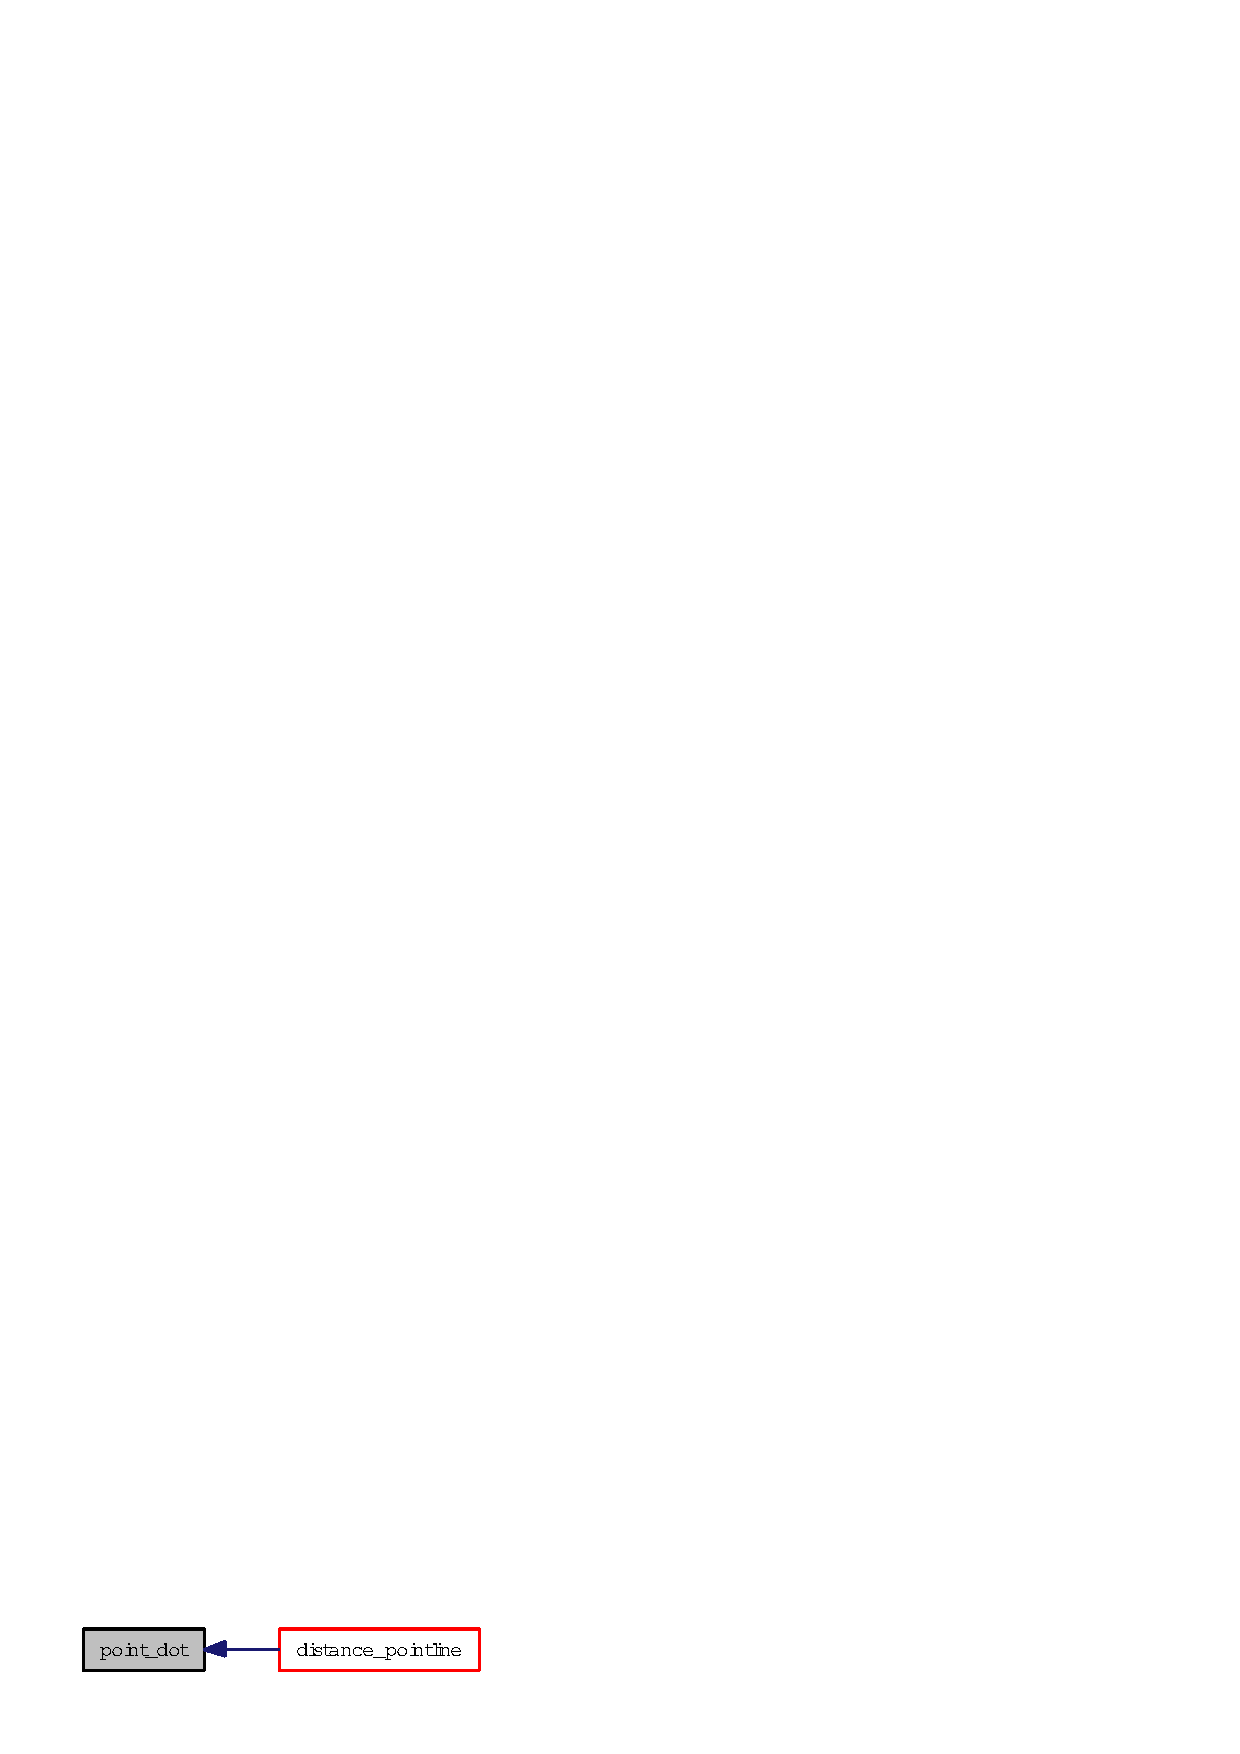
\includegraphics[width=117pt]{group__geometry_ga7ae8d919209fea43e8a61215398bbbe_ga7ae8d919209fea43e8a61215398bbbe_icgraph}
\end{center}
\end{figure}
\hypertarget{group__geometry_gcfbc9e7772d80361768bc0b65cebbca1_gcfbc9e7772d80361768bc0b65cebbca1}{
\index{geometry@{geometry}!polygon_area@{polygon\_\-area}}
\index{polygon_area@{polygon\_\-area}!geometry@{geometry}}
\subsubsection[polygon\_\-area]{\setlength{\rightskip}{0pt plus 5cm}float polygon\_\-area (\hyperlink{struct__polygon}{polygon} $\ast$ {\em p})}}
\label{group__geometry_gcfbc9e7772d80361768bc0b65cebbca1_gcfbc9e7772d80361768bc0b65cebbca1}


Esta funcion calcula el area de un poligono simple, el algoritmo fue tomado de Graphic Gems II, del articulo The Area of a Simple Polygon.

\begin{Desc}
\item[Par\'{a}metros:]
\begin{description}
\item[\mbox{$\leftarrow$} {\em p}]Poligono simple \end{description}
\end{Desc}
\begin{Desc}
\item[Devuelve:]El area del poligono \end{Desc}


Definici\'{o}n en la l\'{\i}nea 20 del archivo polygon.c.

\begin{Code}\begin{verbatim}21 {
22     unsigned int i;
23     float area = 0;
24     for (i=0;i<p->nvertices;i++)
25     {
26         area += p->v[i].x * p->v[(i + 1) % p->nvertices].y;
27         area -= p->v[i].y * p->v[(i + 1) % p->nvertices].x;
28     }
29     area /= 2;
30 
31     return(area < 0 ? -area : area);
32 }
\end{verbatim}\end{Code}




Here is the caller graph for this function:\begin{figure}[H]
\begin{center}
\leavevmode
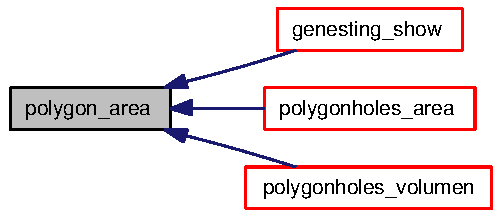
\includegraphics[width=138pt]{group__geometry_gcfbc9e7772d80361768bc0b65cebbca1_gcfbc9e7772d80361768bc0b65cebbca1_icgraph}
\end{center}
\end{figure}
\hypertarget{group__geometry_ge39fef354e4411678ec081c197b29825_ge39fef354e4411678ec081c197b29825}{
\index{geometry@{geometry}!polygon_center@{polygon\_\-center}}
\index{polygon_center@{polygon\_\-center}!geometry@{geometry}}
\subsubsection[polygon\_\-center]{\setlength{\rightskip}{0pt plus 5cm}\hyperlink{struct__point}{point} polygon\_\-center (\hyperlink{struct__polygon}{polygon} $\ast$ {\em p})}}
\label{group__geometry_ge39fef354e4411678ec081c197b29825_ge39fef354e4411678ec081c197b29825}




Definici\'{o}n en la l\'{\i}nea 137 del archivo polygon.c.

\begin{Code}\begin{verbatim}138 {
139     int i=0;
140     float minx, maxx, miny, maxy;
141 
142     point r;
143 
144     polygon_minbox(p, &minx, &miny, &maxx, &maxy)
145 
146     r.x = ((maxx - minx)/2)+minx;
147     r.y = ((maxy - miny)/2)+miny;
148 
149     return r;
150 }
\end{verbatim}\end{Code}




Gr\'{a}fico de llamadas para esta funci\'{o}n:\begin{figure}[H]
\begin{center}
\leavevmode
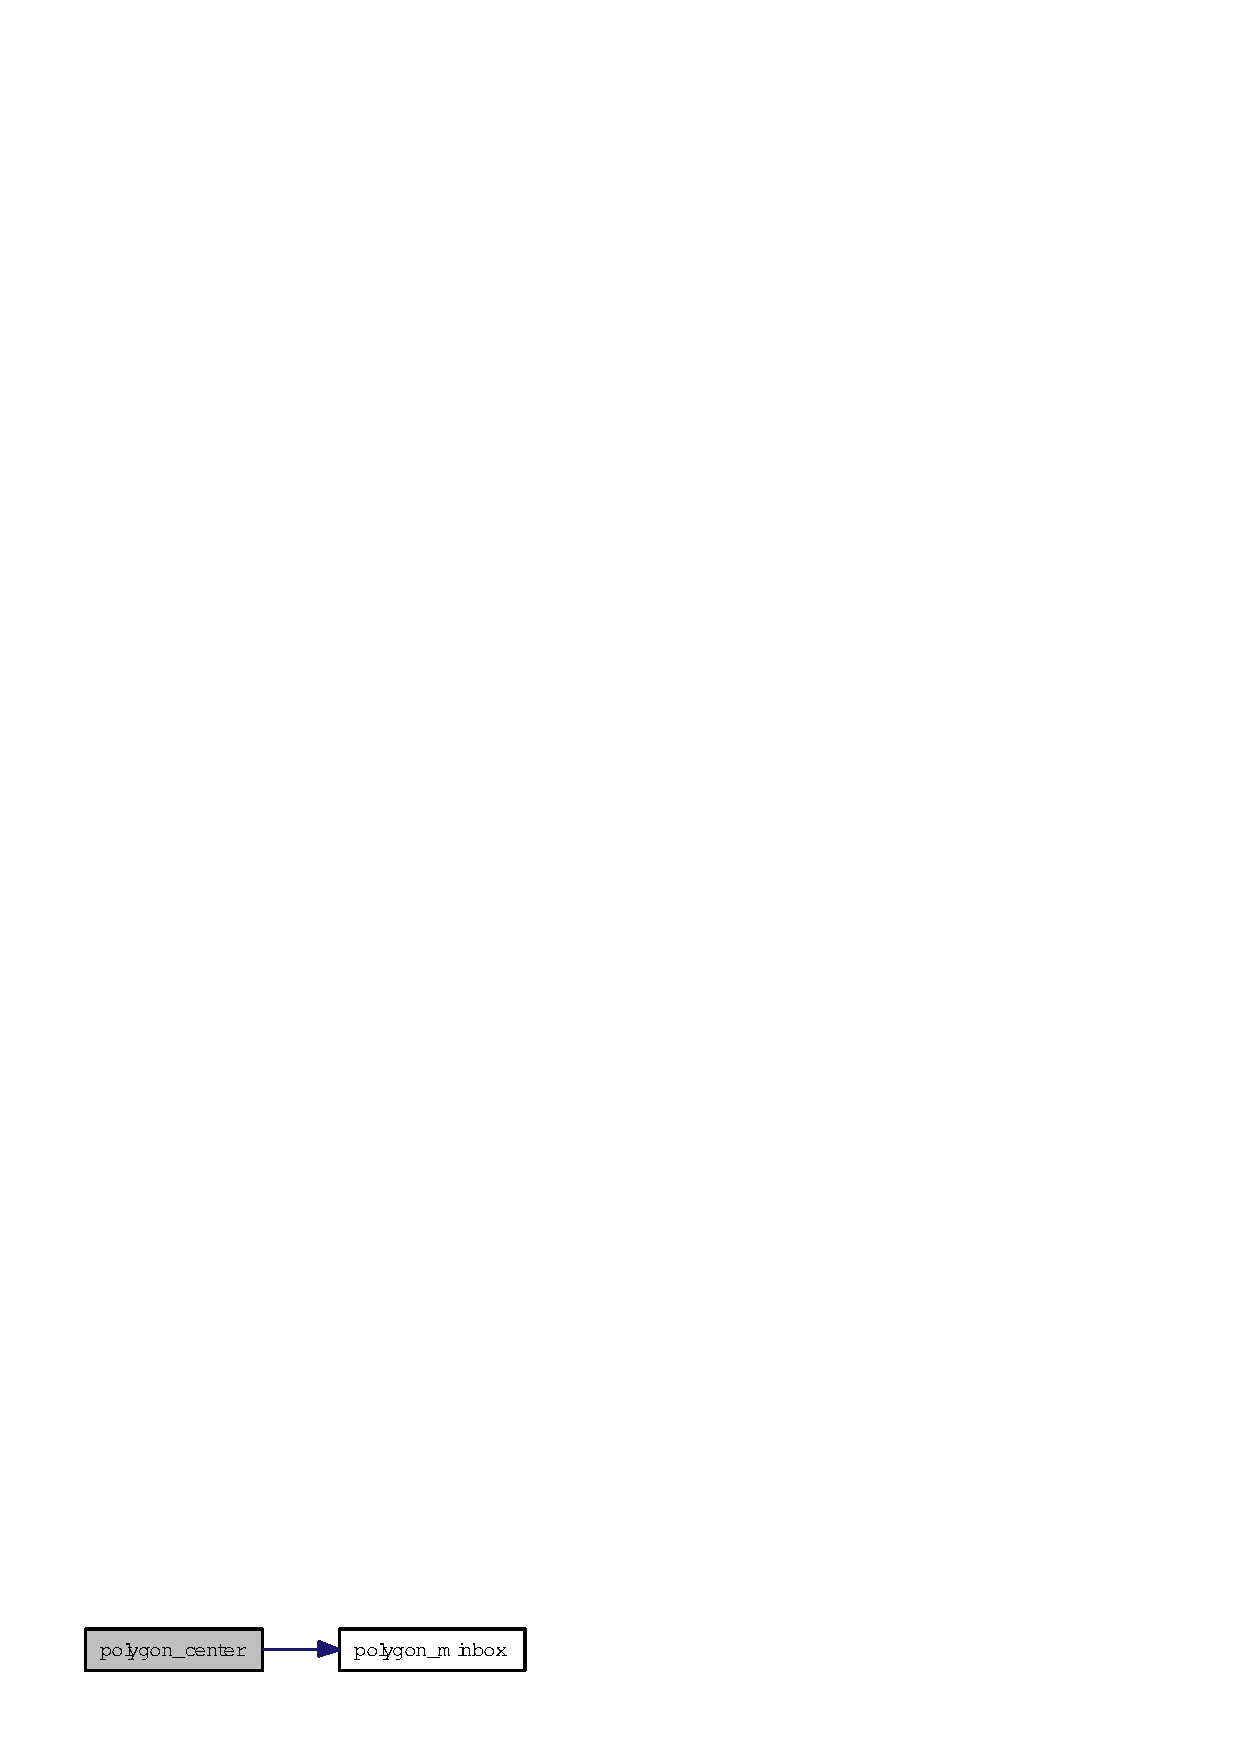
\includegraphics[width=128pt]{group__geometry_ge39fef354e4411678ec081c197b29825_ge39fef354e4411678ec081c197b29825_cgraph}
\end{center}
\end{figure}


Here is the caller graph for this function:\begin{figure}[H]
\begin{center}
\leavevmode
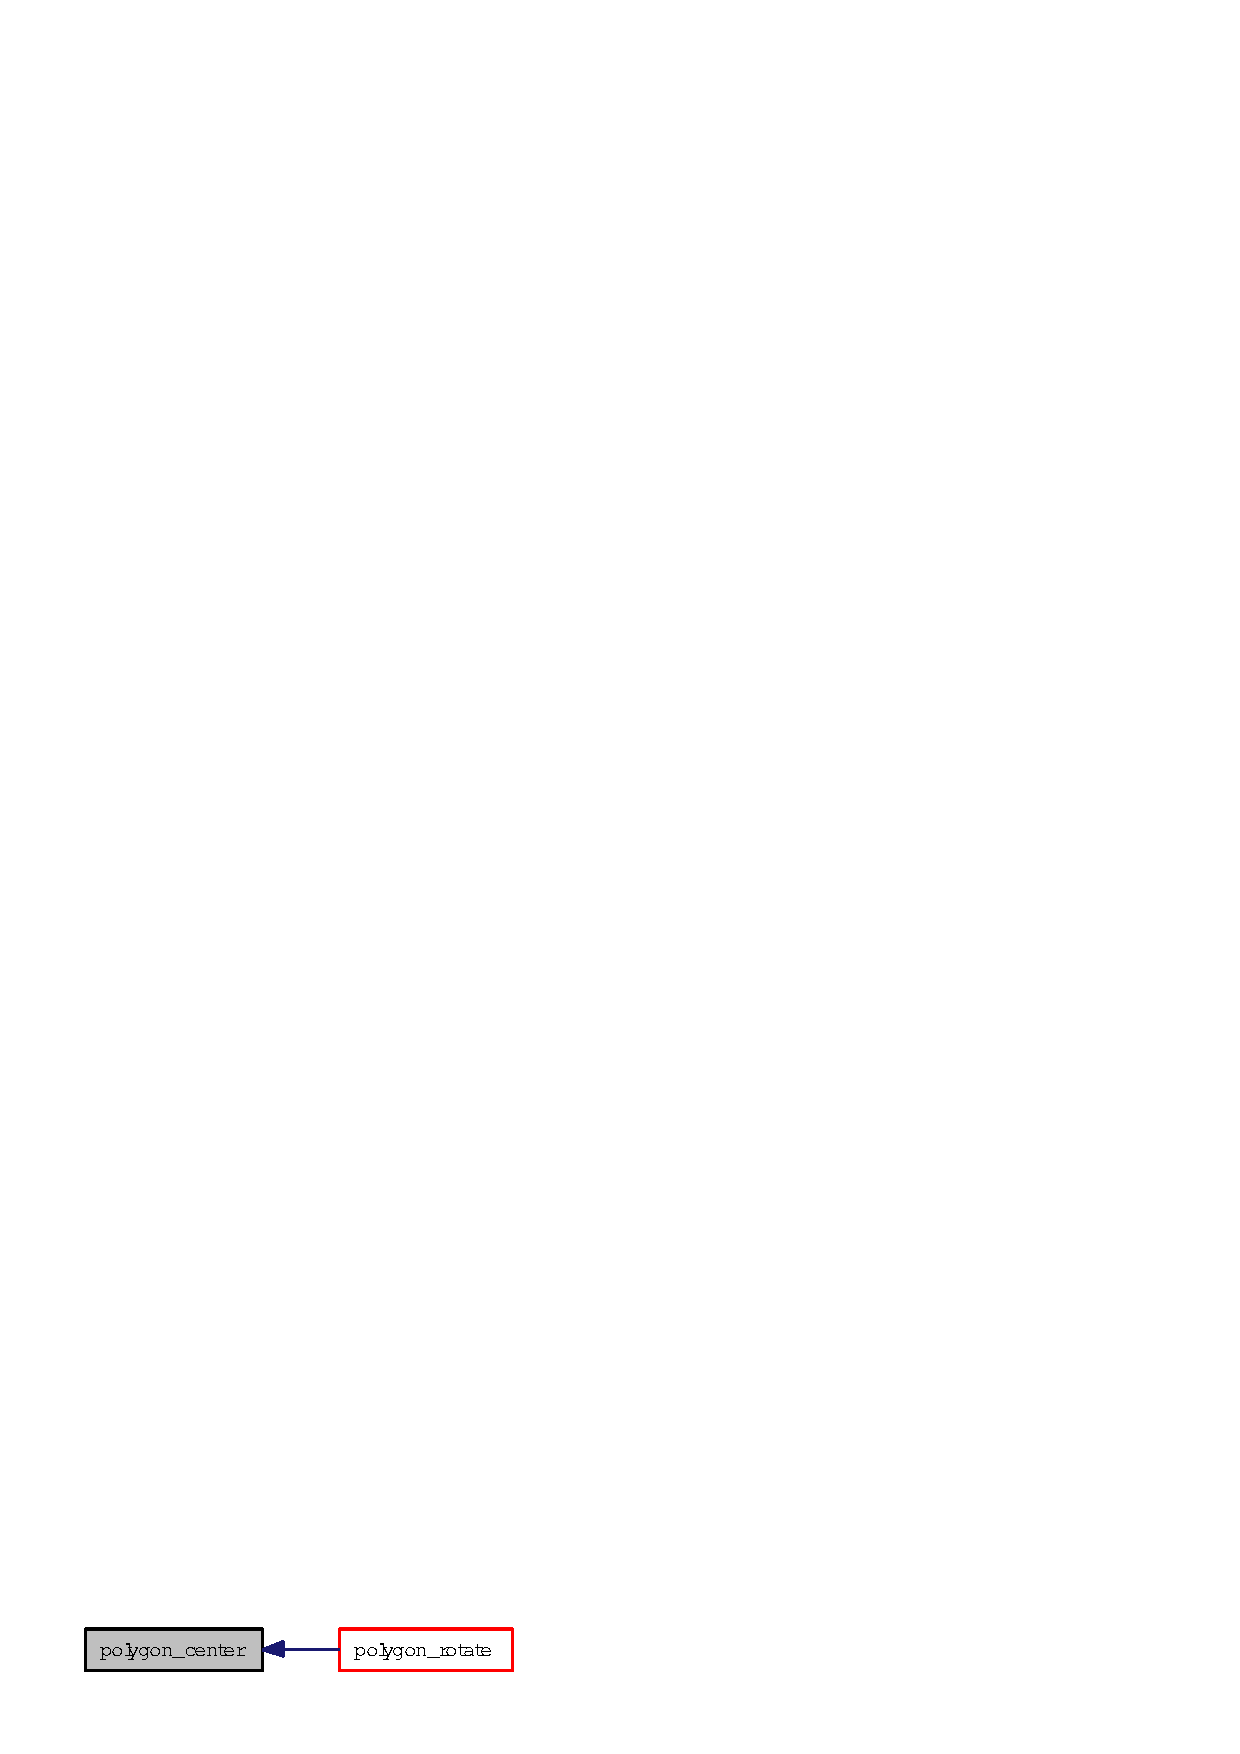
\includegraphics[width=125pt]{group__geometry_ge39fef354e4411678ec081c197b29825_ge39fef354e4411678ec081c197b29825_icgraph}
\end{center}
\end{figure}
\hypertarget{group__geometry_g137ef6f552a0a04c5ae0493690088f3f_g137ef6f552a0a04c5ae0493690088f3f}{
\index{geometry@{geometry}!polygon_minbox@{polygon\_\-minbox}}
\index{polygon_minbox@{polygon\_\-minbox}!geometry@{geometry}}
\subsubsection[polygon\_\-minbox]{\setlength{\rightskip}{0pt plus 5cm}void polygon\_\-minbox (\hyperlink{struct__polygon}{polygon} $\ast$ {\em p}, float $\ast$ {\em minx}, float $\ast$ {\em miny}, float $\ast$ {\em maxx}, float $\ast$ {\em maxy})}}
\label{group__geometry_g137ef6f552a0a04c5ae0493690088f3f_g137ef6f552a0a04c5ae0493690088f3f}


La funcion calcula las coordenadas mas extremas del poligono, conformando con estas 2 puntos que pueden formar un rectangulo que contiene completamente el poligono

\begin{Desc}
\item[Par\'{a}metros:]
\begin{description}
\item[\mbox{$\leftarrow$} {\em p}]Poligono simple \item[\mbox{$\rightarrow$} {\em minx}]Coordenada mas peque\~{n}a del poligono en el eje x \item[\mbox{$\rightarrow$} {\em miny}]Coordenada mas peque\~{n}a del poligono en el eje y \item[\mbox{$\rightarrow$} {\em maxx}]Coordenada mas grande del poligono en el eje x \item[\mbox{$\rightarrow$} {\em maxy}]Coordenada mas grande del poligono en el eje y \end{description}
\end{Desc}


Definici\'{o}n en la l\'{\i}nea 163 del archivo polygon.c.

\begin{Code}\begin{verbatim}164 {
165     int i;
166 
167     *minx = p->v[0].x;
168     *miny = p->v[0].y;
169     *maxx = p->v[0].x;
170     *maxy = p->v[0].y;
171 
172     for (i=1;i<p->nvertices;i++)
173     {
174         if (*minx > p->v[i].x)
175         {
176             *minx = p->v[i].x;
177         }
178         if (*miny > p->v[i].y)
179         {
180             *miny = p->v[i].y;
181         }
182         if (*maxx < p->v[i].x)
183         {
184             *maxx = p->v[i].x;
185         }
186         if (*maxy < p->v[i].y)
187         {
188             *maxy = p->v[i].y;
189         }
190     }
191 }
\end{verbatim}\end{Code}




Here is the caller graph for this function:\begin{figure}[H]
\begin{center}
\leavevmode
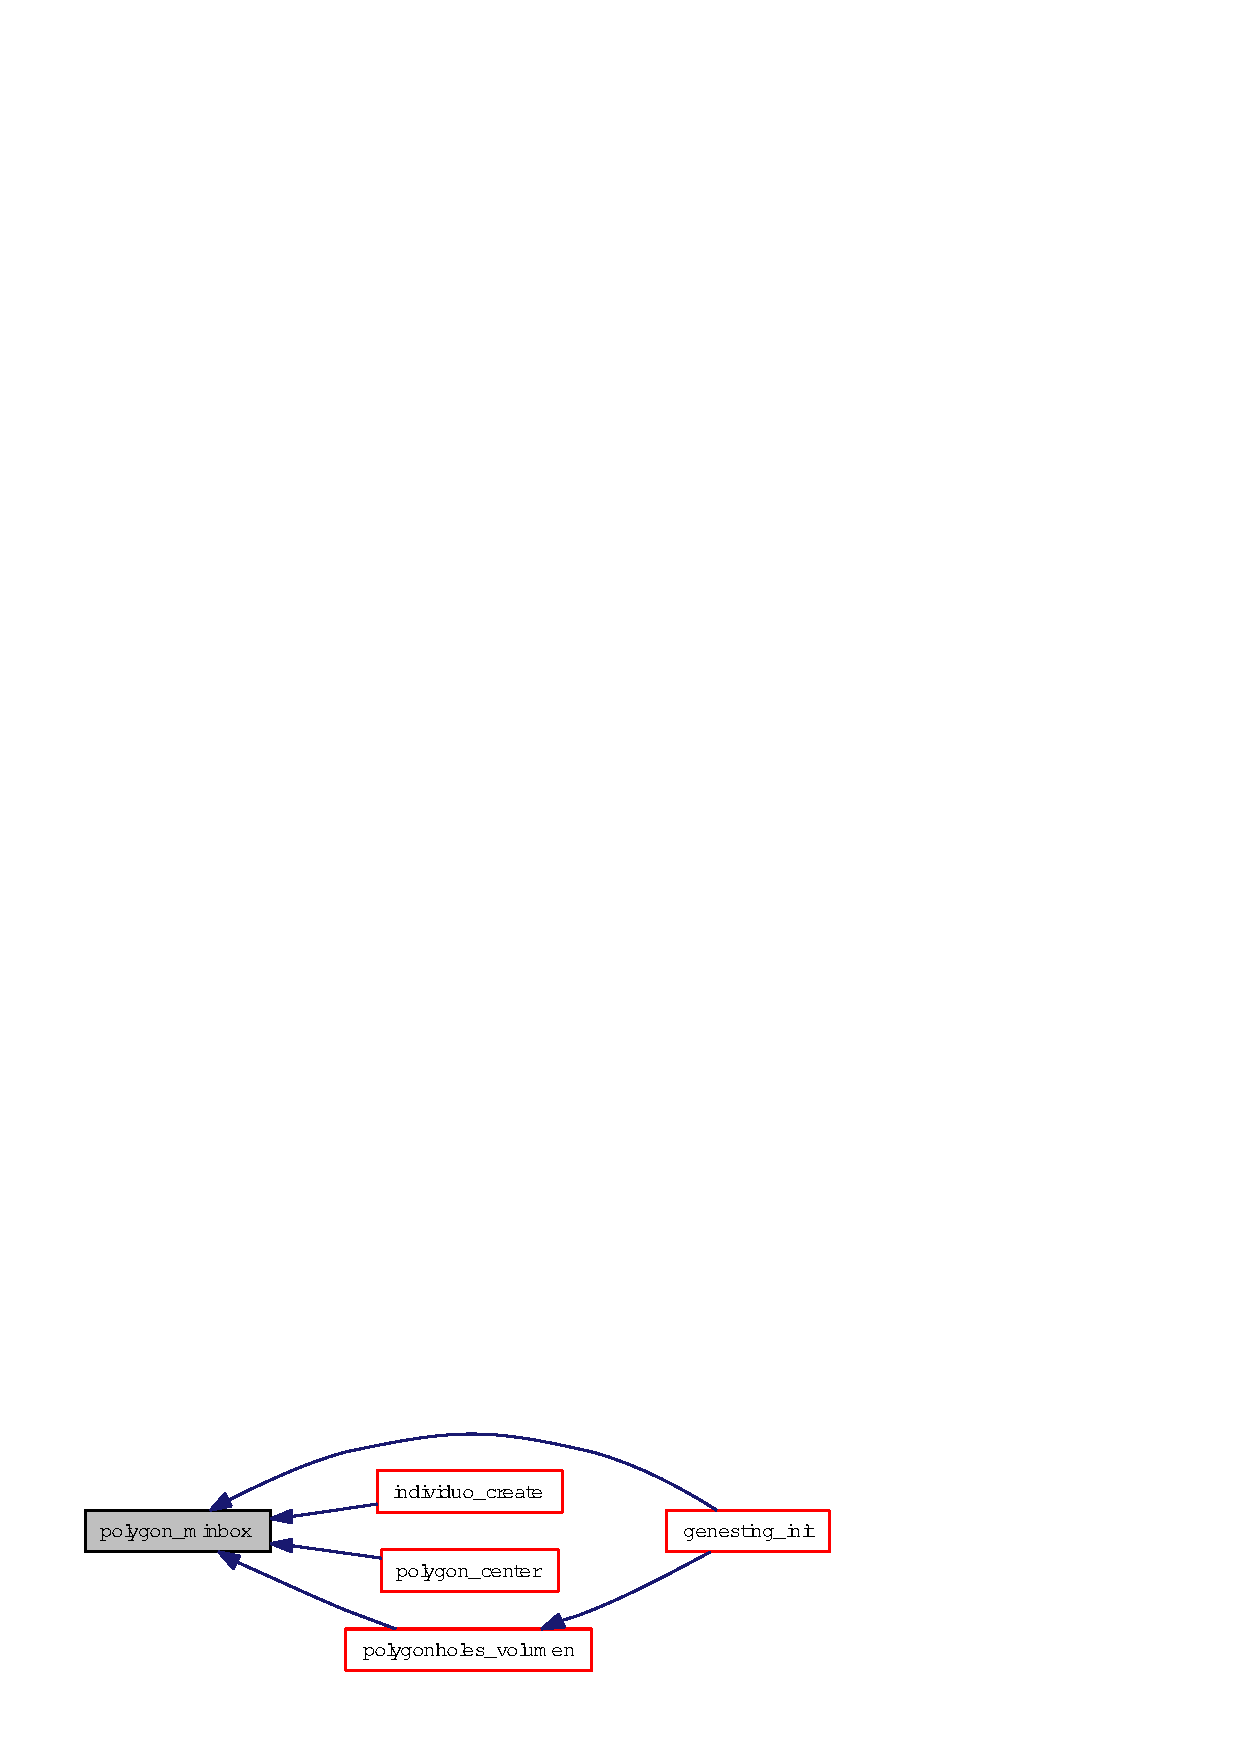
\includegraphics[width=201pt]{group__geometry_g137ef6f552a0a04c5ae0493690088f3f_g137ef6f552a0a04c5ae0493690088f3f_icgraph}
\end{center}
\end{figure}
\hypertarget{group__geometry_g2be6101a257ea8896e61e93d14b22b89_g2be6101a257ea8896e61e93d14b22b89}{
\index{geometry@{geometry}!polygon_overlapping@{polygon\_\-overlapping}}
\index{polygon_overlapping@{polygon\_\-overlapping}!geometry@{geometry}}
\subsubsection[polygon\_\-overlapping]{\setlength{\rightskip}{0pt plus 5cm}bool polygon\_\-overlapping (\hyperlink{struct__polygon}{polygon} $\ast$ {\em p}, \hyperlink{struct__polygon}{polygon} $\ast$ {\em q})}}
\label{group__geometry_g2be6101a257ea8896e61e93d14b22b89_g2be6101a257ea8896e61e93d14b22b89}


Esta funcion identifica si dos poligonos se solapan de alguna forma para verificar esto se realizan 3 comprobaciones:\begin{itemize}
\item Ningun vertice del poligono p esta dentro del poligono q\item Ningun vertice del poligono q esta dentro del poligono p\item Ninguna linea de los poligonos p y q se intersectan\end{itemize}


\begin{Desc}
\item[Par\'{a}metros:]
\begin{description}
\item[\mbox{$\leftarrow$} {\em p}]Poligono Simple en 2 dimensiones \item[\mbox{$\leftarrow$} {\em q}]Poligono Simple en 2 dimensiones \end{description}
\end{Desc}
\begin{Desc}
\item[Devuelve:]Verdadero si los poligonos se solapan, falso en caso contrario. \end{Desc}


Definici\'{o}n en la l\'{\i}nea 74 del archivo polygon.c.

\begin{Code}\begin{verbatim}75 {
76     int i,j;
77 
78     for (i=0;i<p->nvertices;i++)
79     {
80         if (polygon_pointin(q,&p->v[i]))
81             return true;
82     }
83 
84     for (i=0;i<q->nvertices;i++)
85     {
86         if (polygon_pointin(p,&q->v[i]))
87             return true;
88     }
89 
90     for (i=0;i<p->nvertices;i++)
91     {
92         line t1,t2;
93         t1.v1=p->v[i];
94         t1.v2=p->v[(i+1)%(p->nvertices)];
95         for (j=0;j<q->nvertices;j++)
96         {
97             t2.v1=q->v[j];
98             t2.v2=q->v[(j+1)%q->nvertices];
99             if (line_intersection(&t1,&t2))
100                 return true;
101         }
102     }
103     return false;
104 }
\end{verbatim}\end{Code}




Gr\'{a}fico de llamadas para esta funci\'{o}n:\begin{figure}[H]
\begin{center}
\leavevmode
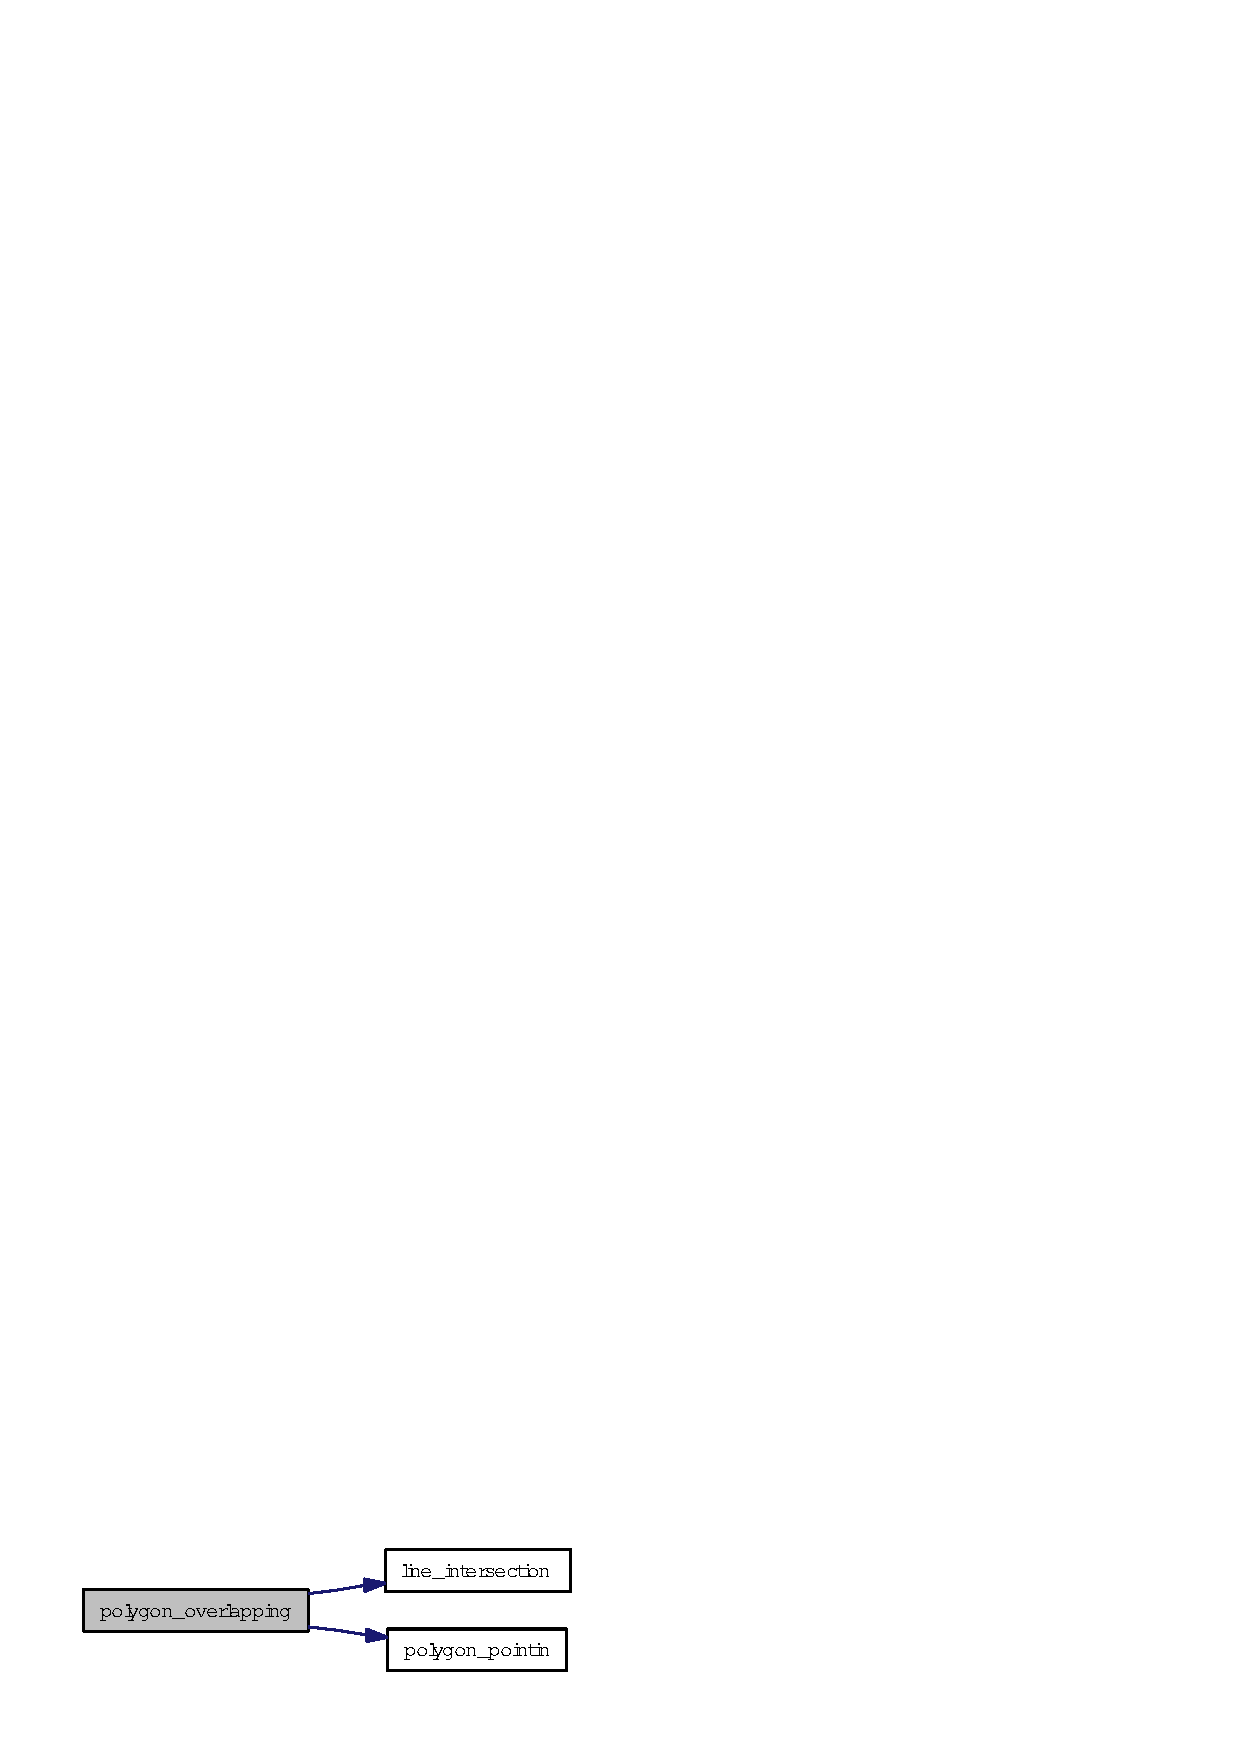
\includegraphics[width=139pt]{group__geometry_g2be6101a257ea8896e61e93d14b22b89_g2be6101a257ea8896e61e93d14b22b89_cgraph}
\end{center}
\end{figure}


Here is the caller graph for this function:\begin{figure}[H]
\begin{center}
\leavevmode
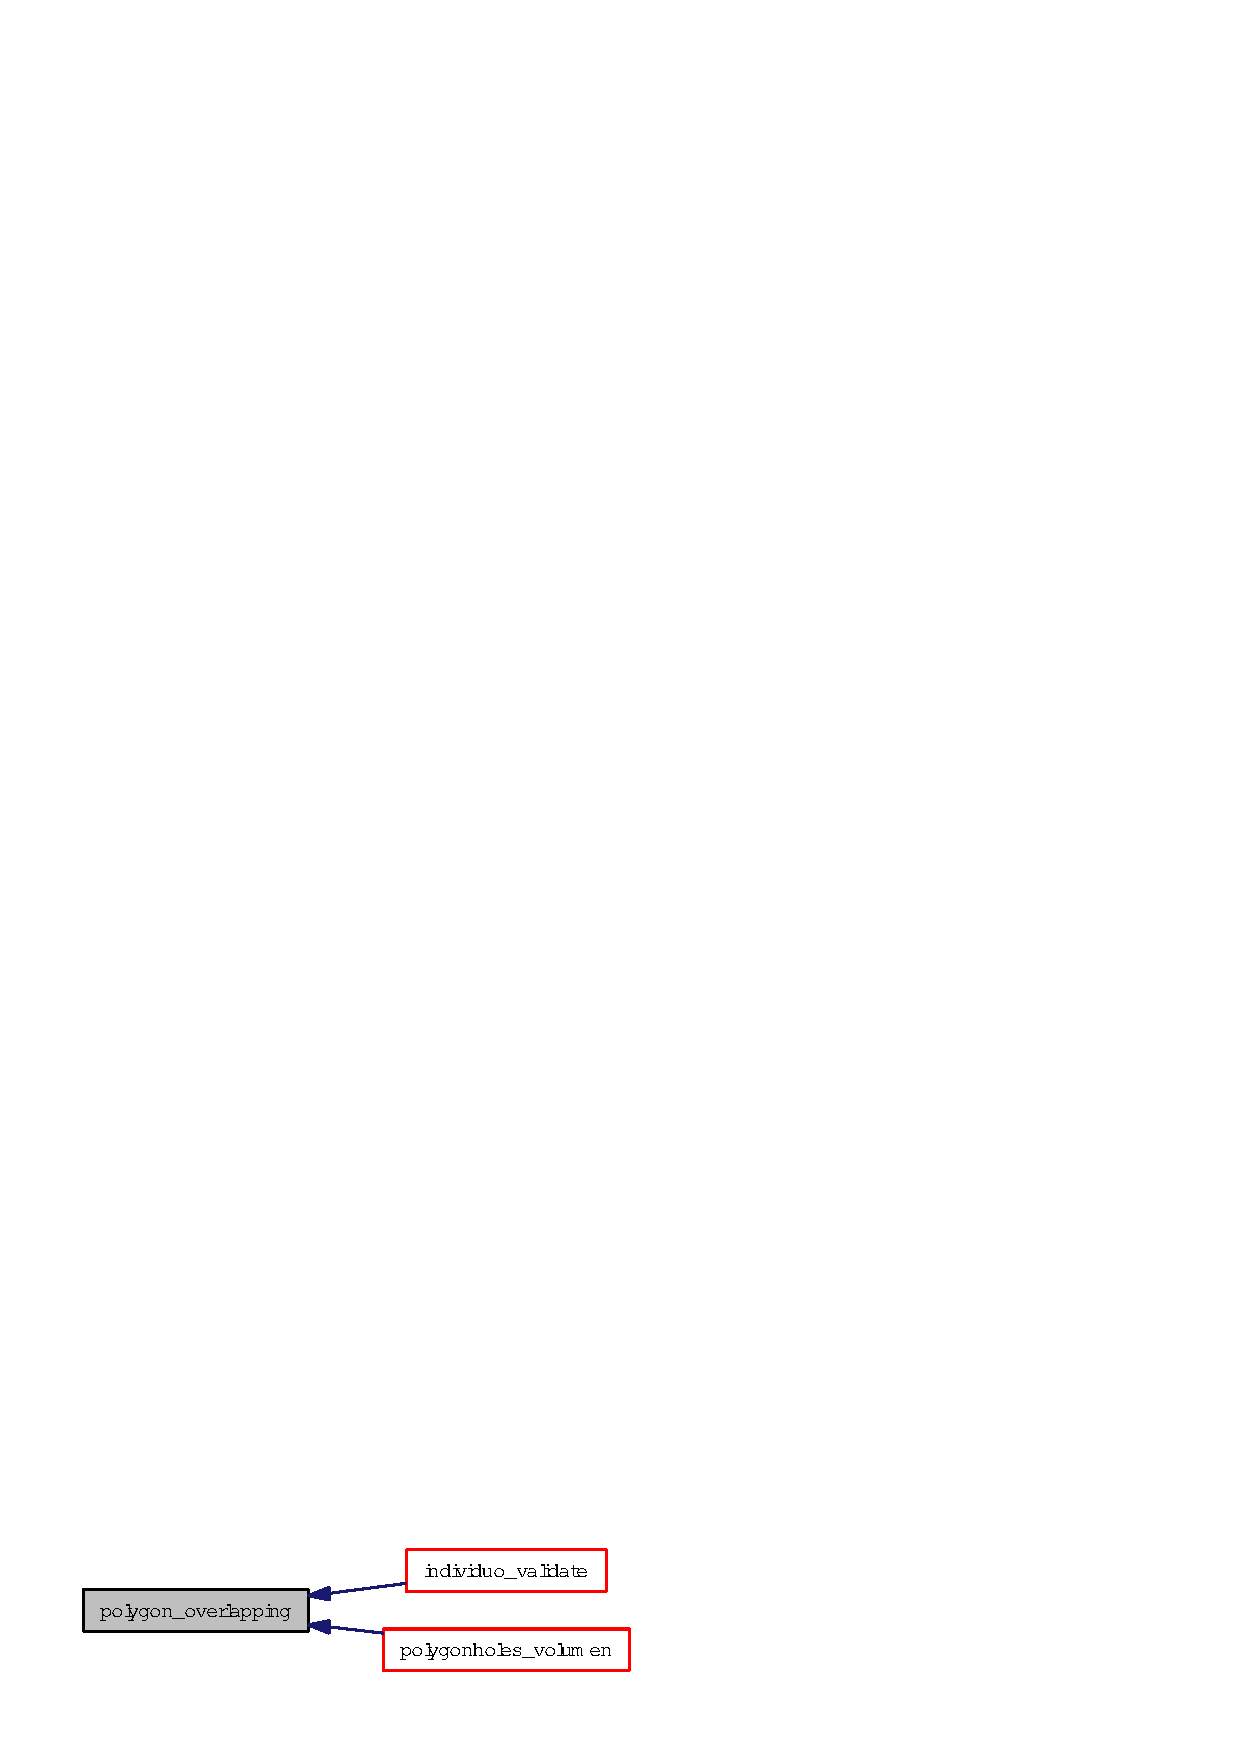
\includegraphics[width=153pt]{group__geometry_g2be6101a257ea8896e61e93d14b22b89_g2be6101a257ea8896e61e93d14b22b89_icgraph}
\end{center}
\end{figure}
\hypertarget{group__geometry_geab0a1d6da7c44ae49494958bb885504_geab0a1d6da7c44ae49494958bb885504}{
\index{geometry@{geometry}!polygon_pointin@{polygon\_\-pointin}}
\index{polygon_pointin@{polygon\_\-pointin}!geometry@{geometry}}
\subsubsection[polygon\_\-pointin]{\setlength{\rightskip}{0pt plus 5cm}bool polygon\_\-pointin (\hyperlink{struct__polygon}{polygon} $\ast$ {\em p}, \hyperlink{struct__point}{point} $\ast$ {\em f})}}
\label{group__geometry_geab0a1d6da7c44ae49494958bb885504_geab0a1d6da7c44ae49494958bb885504}


La funcion identifica si un punto esta dentro de un poligono o no.

\begin{Desc}
\item[Par\'{a}metros:]
\begin{description}
\item[\mbox{$\leftarrow$} {\em p}]Poligono simple en 2 dimensiones \item[\mbox{$\leftarrow$} {\em f}]Punto en 2 dimensiones \end{description}
\end{Desc}
\begin{Desc}
\item[Devuelve:]Un booleano que es verdadero en caso de que el punto este dentro del poligono y falso en caso contrario \end{Desc}


Definici\'{o}n en la l\'{\i}nea 48 del archivo polygon.c.

\begin{Code}\begin{verbatim}49 {
50     bool c=false;
51     unsigned int i,j;
52 
53     for (i=0,j=p->nvertices-1;i<p->nvertices;j=i++)
54     {
55         if ((((p->v[i].y<=f->y) && (f->y<p->v[j].y)) ||
56                 ((p->v[j].y<=f->y) && (f->y<p->v[i].y))) &&
57                 (f->x < (p->v[j].x - p->v[i].x) * (f->y - p->v[i].y) / (p->v[j].y - p->v[i].y) + p->v[i].x))
58             c = !c;
59     }
60     return c;
61 }
\end{verbatim}\end{Code}




Here is the caller graph for this function:\begin{figure}[H]
\begin{center}
\leavevmode
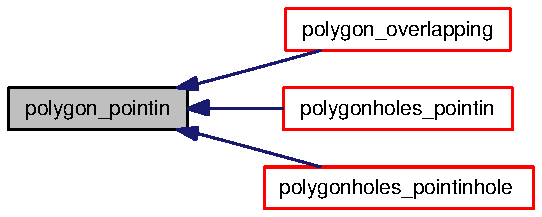
\includegraphics[width=148pt]{group__geometry_geab0a1d6da7c44ae49494958bb885504_geab0a1d6da7c44ae49494958bb885504_icgraph}
\end{center}
\end{figure}
\hypertarget{group__geometry_g95276abee7240f116afaf80a3e1f23c4_g95276abee7240f116afaf80a3e1f23c4}{
\index{geometry@{geometry}!polygon_rotate@{polygon\_\-rotate}}
\index{polygon_rotate@{polygon\_\-rotate}!geometry@{geometry}}
\subsubsection[polygon\_\-rotate]{\setlength{\rightskip}{0pt plus 5cm}void polygon\_\-rotate (\hyperlink{struct__polygon}{polygon} $\ast$ {\em p}, float {\em t})}}
\label{group__geometry_g95276abee7240f116afaf80a3e1f23c4_g95276abee7240f116afaf80a3e1f23c4}


La funcion rota el poligono p un angulo t, teniendo como eje de rotacion el centro de la caja mas pequena que contiene el poligono. Aunque se pueden elegir otros puntos como eje, o de hecho implementar un eje arbitrario, el centro de la caja que contiene el poligono es un punto facil de calcular y ademas que evita exageradas translaciones relativas del poligono al ser rotado.

\begin{Desc}
\item[Par\'{a}metros:]
\begin{description}
\item[\mbox{$\leftrightarrow$} {\em p}]Poligono simple \item[\mbox{$\leftarrow$} {\em t}]Angulo en radianes a rotar la figura en sentido antihorario. \end{description}
\end{Desc}


Definici\'{o}n en la l\'{\i}nea 116 del archivo polygon.c.

\begin{Code}\begin{verbatim}117 {
118     int i;
119     point pc;
120 
121     float sent = sin(t);
122     float cost = cos(t);
123 
124     pc = polygon_center(p);
125 
126     polygon_translate(p, -pc.x, -pc.y);
127 
128     for (i=0;i<p->nvertices;i++)
129     {
130         p->v[i].x=(p->v[i].x*cost - p->v[i].y * sent);
131         p->v[i].y=(p->v[i].y*cost + p->v[i].x * sent);
132     }
133 
134     polygon_translate(p, pc.x, pc.y);
135 }
\end{verbatim}\end{Code}




Gr\'{a}fico de llamadas para esta funci\'{o}n:\begin{figure}[H]
\begin{center}
\leavevmode
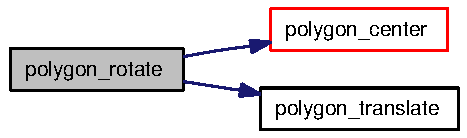
\includegraphics[width=130pt]{group__geometry_g95276abee7240f116afaf80a3e1f23c4_g95276abee7240f116afaf80a3e1f23c4_cgraph}
\end{center}
\end{figure}


Here is the caller graph for this function:\begin{figure}[H]
\begin{center}
\leavevmode
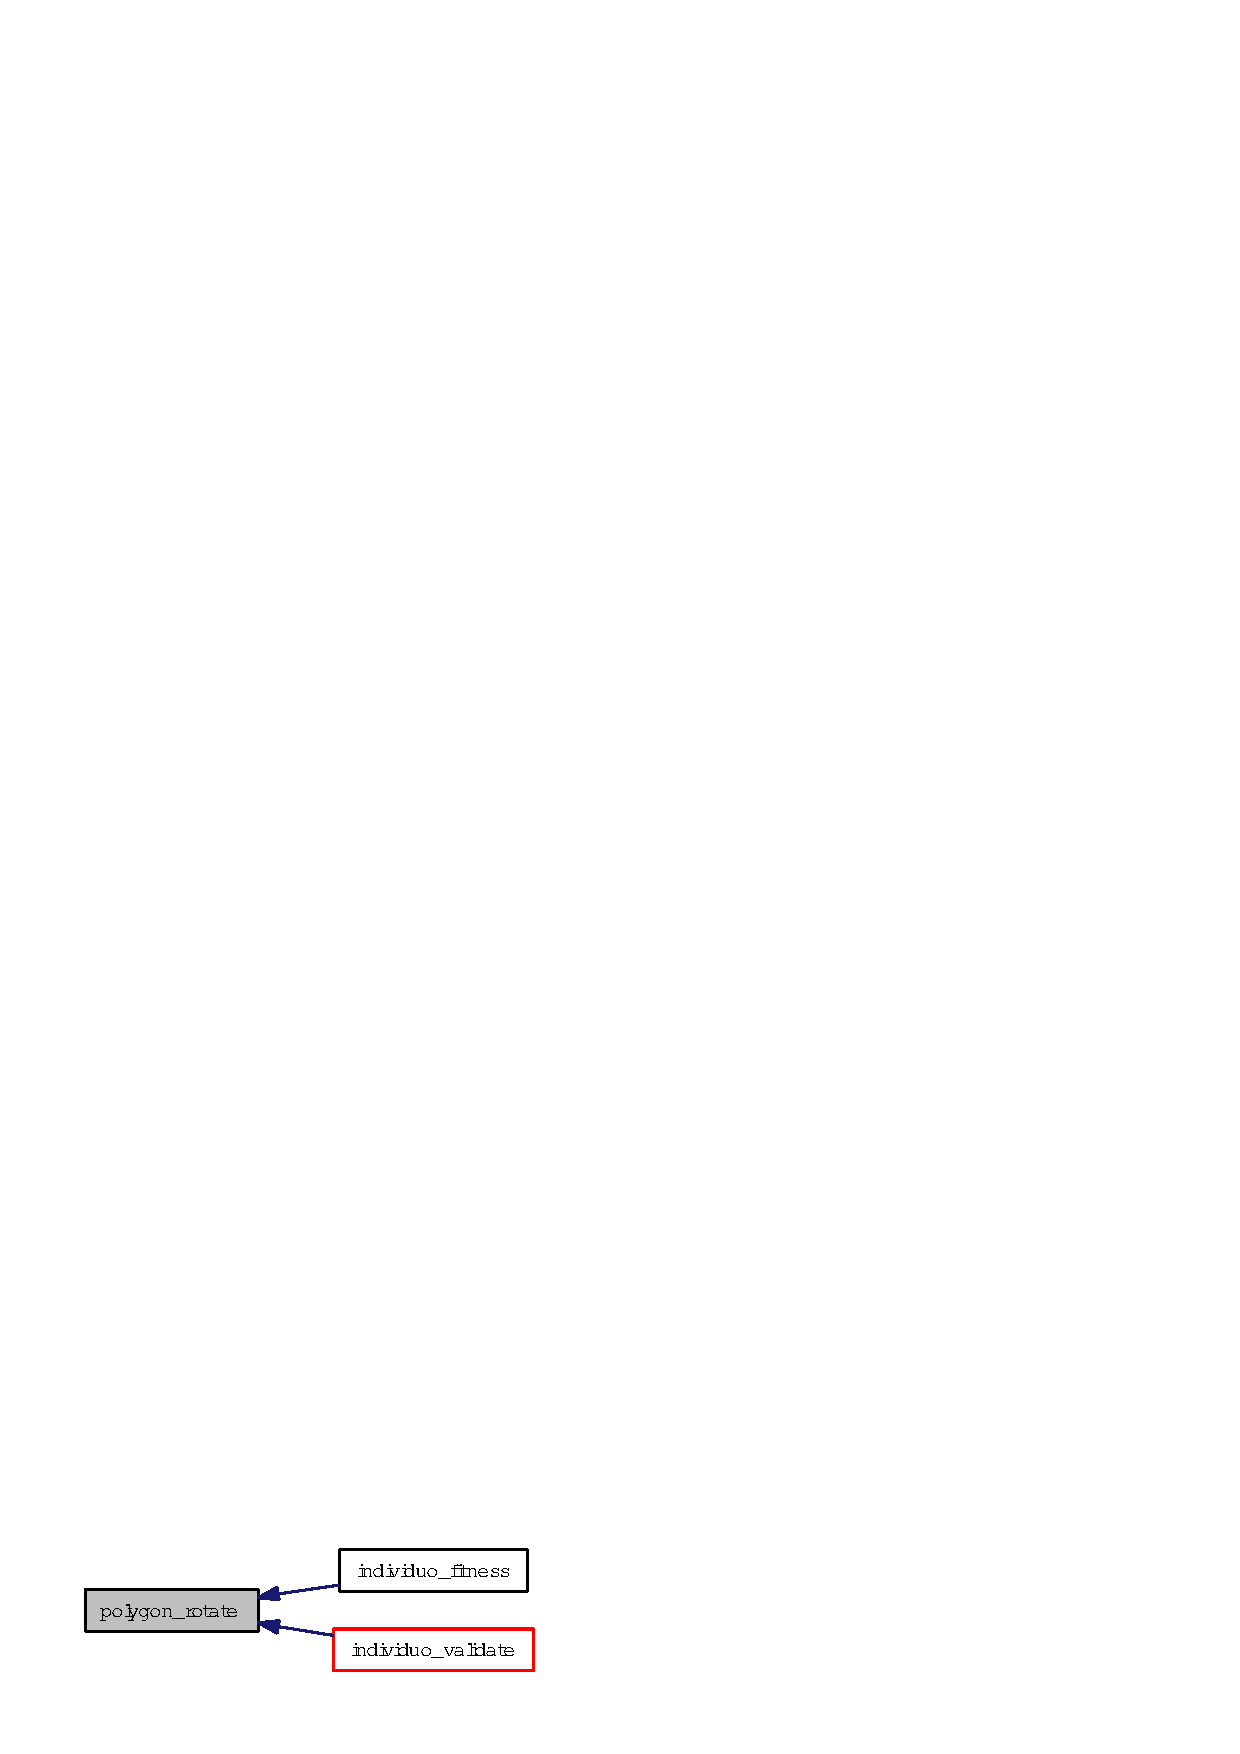
\includegraphics[width=130pt]{group__geometry_g95276abee7240f116afaf80a3e1f23c4_g95276abee7240f116afaf80a3e1f23c4_icgraph}
\end{center}
\end{figure}
\hypertarget{group__geometry_g7538c2bf0d1e8acc0cfc055b6bf3a96b_g7538c2bf0d1e8acc0cfc055b6bf3a96b}{
\index{geometry@{geometry}!polygon_translate@{polygon\_\-translate}}
\index{polygon_translate@{polygon\_\-translate}!geometry@{geometry}}
\subsubsection[polygon\_\-translate]{\setlength{\rightskip}{0pt plus 5cm}void polygon\_\-translate (\hyperlink{struct__polygon}{polygon} $\ast$ {\em p}, float {\em x}, float {\em y})}}
\label{group__geometry_g7538c2bf0d1e8acc0cfc055b6bf3a96b_g7538c2bf0d1e8acc0cfc055b6bf3a96b}


Translada el poligono una distancia definida por x,y.

\begin{Desc}
\item[Par\'{a}metros:]
\begin{description}
\item[\mbox{$\leftrightarrow$} {\em p}]Poligono simple \item[\mbox{$\leftarrow$} {\em x}]Distancia en x a transladar el poligono \item[\mbox{$\leftarrow$} {\em y}]Distancia en y a transladar el poligono \end{description}
\end{Desc}


Definici\'{o}n en la l\'{\i}nea 200 del archivo polygon.c.

\begin{Code}\begin{verbatim}201 {
202     int i;
203     for (i=0;i<p->nvertices;i++)
204     {
205         p->v[i].x+=x;
206         p->v[i].y+=y;
207     }
208 }
\end{verbatim}\end{Code}




Here is the caller graph for this function:\begin{figure}[H]
\begin{center}
\leavevmode
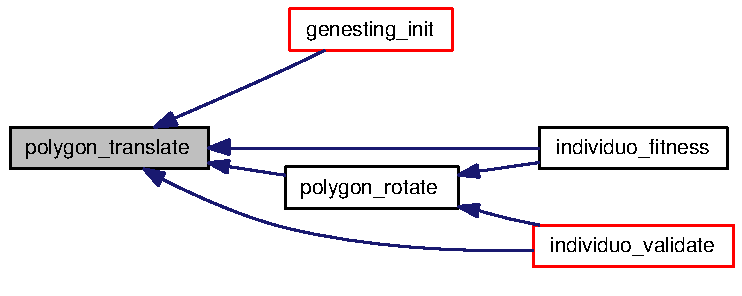
\includegraphics[width=196pt]{group__geometry_g7538c2bf0d1e8acc0cfc055b6bf3a96b_g7538c2bf0d1e8acc0cfc055b6bf3a96b_icgraph}
\end{center}
\end{figure}
\hypertarget{group__geometry_g380cdcfa6caf51828c8d06f4518a4084_g380cdcfa6caf51828c8d06f4518a4084}{
\index{geometry@{geometry}!polygonholes_area@{polygonholes\_\-area}}
\index{polygonholes_area@{polygonholes\_\-area}!geometry@{geometry}}
\subsubsection[polygonholes\_\-area]{\setlength{\rightskip}{0pt plus 5cm}float polygonholes\_\-area (\hyperlink{struct__polygon__holes}{polygon\_\-holes} $\ast$ {\em p})}}
\label{group__geometry_g380cdcfa6caf51828c8d06f4518a4084_g380cdcfa6caf51828c8d06f4518a4084}


La funcion calcula el area de un Poligono con huecos, para hacer esto calculamos el area del poligono formado por el borde exterior y le restamos el area de cada uno de los huecos.

\begin{Desc}
\item[Par\'{a}metros:]
\begin{description}
\item[\mbox{$\leftarrow$} {\em p}]Poligono simple en 2 dimensiones \end{description}
\end{Desc}
\begin{Desc}
\item[Devuelve:]Area del poligono simple con huecos \end{Desc}


Definici\'{o}n en la l\'{\i}nea 30 del archivo polygon\_\-holes.c.

\begin{Code}\begin{verbatim}31 {
32     unsigned int i;
33     float area;
34     area = polygon_area(p->p);
35     for (i=0;i<p->nholes;i++)
36     {
37         area -= polygon_area(&(p->h[i]));
38     }
39     return area;
40 }
\end{verbatim}\end{Code}




Gr\'{a}fico de llamadas para esta funci\'{o}n:\begin{figure}[H]
\begin{center}
\leavevmode
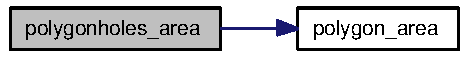
\includegraphics[width=130pt]{group__geometry_g380cdcfa6caf51828c8d06f4518a4084_g380cdcfa6caf51828c8d06f4518a4084_cgraph}
\end{center}
\end{figure}


Here is the caller graph for this function:\begin{figure}[H]
\begin{center}
\leavevmode
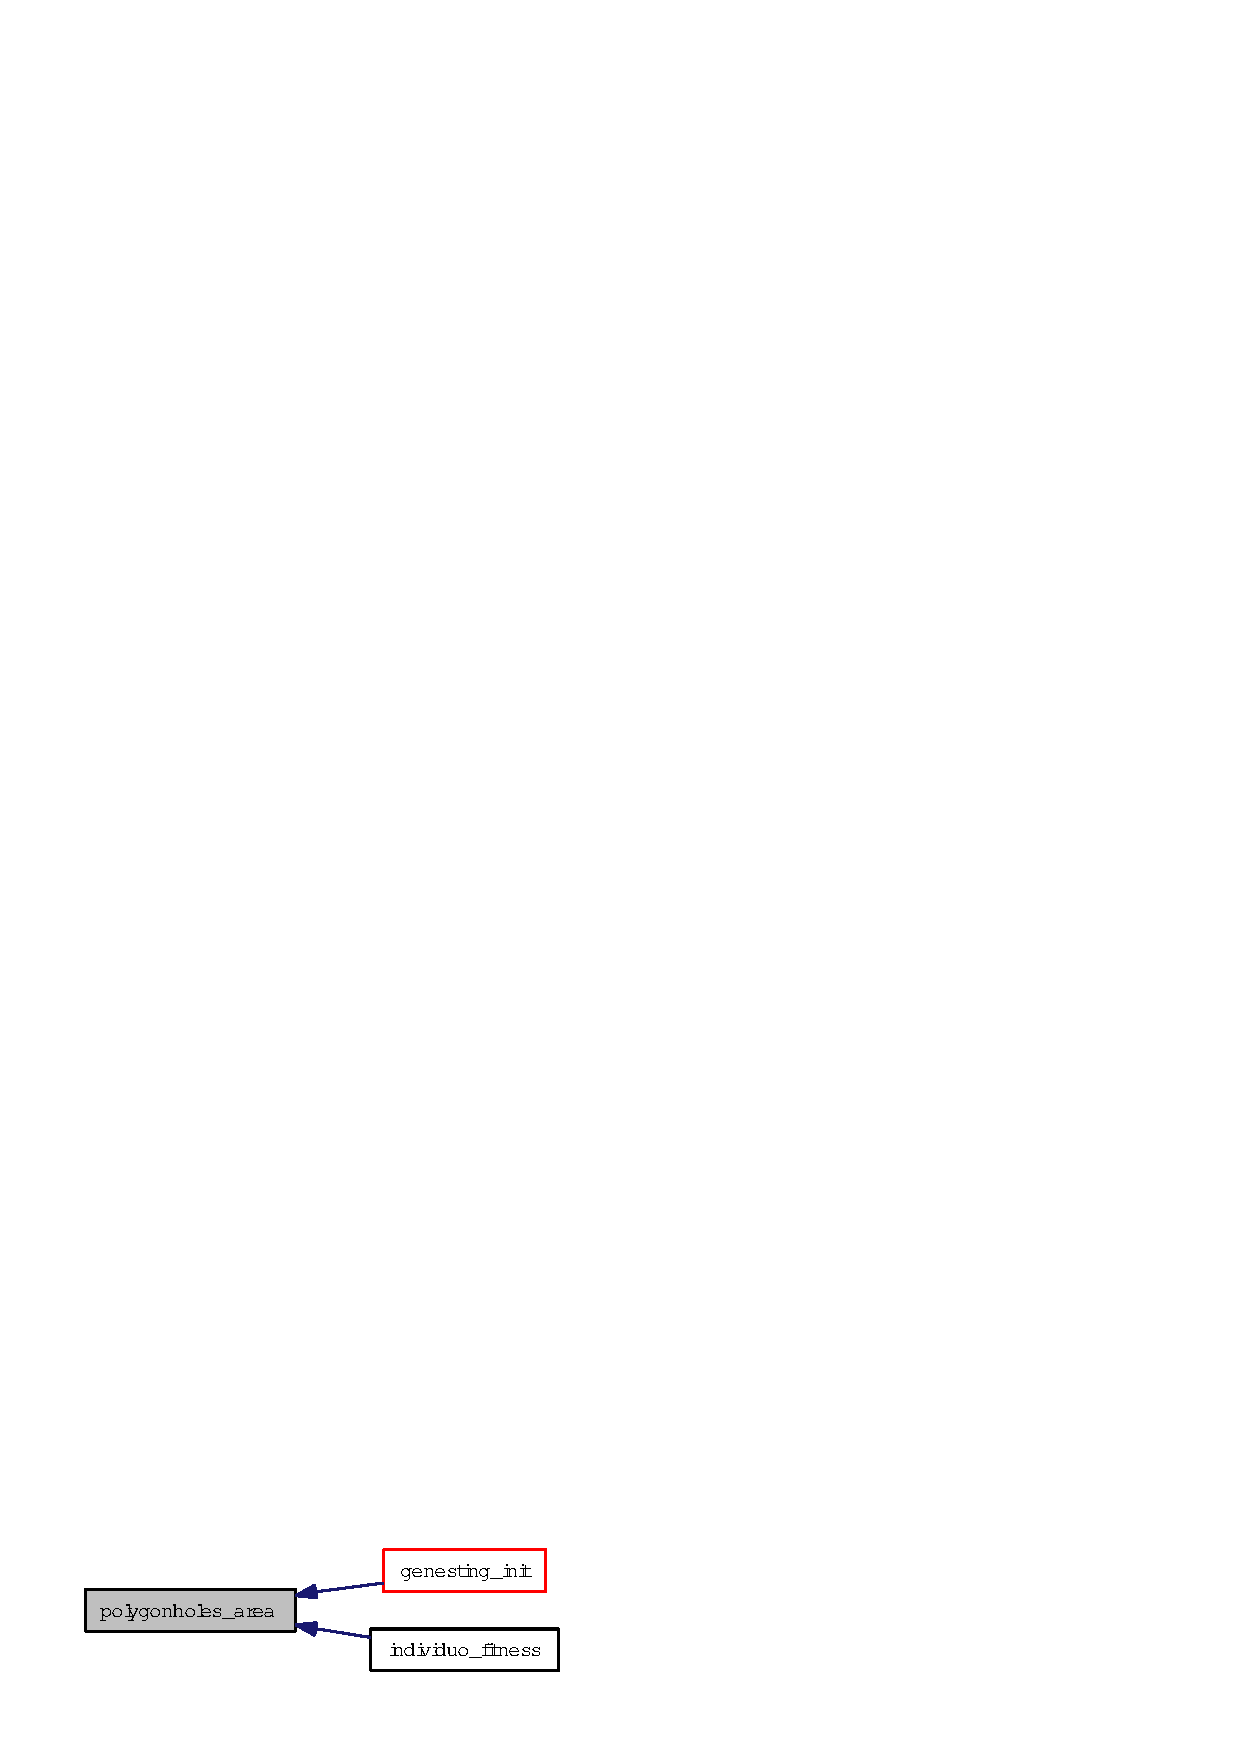
\includegraphics[width=136pt]{group__geometry_g380cdcfa6caf51828c8d06f4518a4084_g380cdcfa6caf51828c8d06f4518a4084_icgraph}
\end{center}
\end{figure}
\hypertarget{group__geometry_g35a6dd45f6d0cbed26ef8a69ed34a2e9_g35a6dd45f6d0cbed26ef8a69ed34a2e9}{
\index{geometry@{geometry}!polygonholes_pointin@{polygonholes\_\-pointin}}
\index{polygonholes_pointin@{polygonholes\_\-pointin}!geometry@{geometry}}
\subsubsection[polygonholes\_\-pointin]{\setlength{\rightskip}{0pt plus 5cm}bool polygonholes\_\-pointin (\hyperlink{struct__polygon__holes}{polygon\_\-holes} $\ast$ {\em p}, \hyperlink{struct__point}{point} $\ast$ {\em f})}}
\label{group__geometry_g35a6dd45f6d0cbed26ef8a69ed34a2e9_g35a6dd45f6d0cbed26ef8a69ed34a2e9}


Esta funcion identifica si un punto esta dentro de un poligono con huecos por lo tanto evalua inicialmente que el punto este dentro del poligono exterior y posterioremente que no se encuentre dentro de los huecos

\begin{Desc}
\item[Par\'{a}metros:]
\begin{description}
\item[\mbox{$\leftarrow$} {\em p}]Poligono simple con huecos en 2 dimensiones \item[\mbox{$\leftarrow$} {\em f}]Punto en 2 dimensiones \end{description}
\end{Desc}
\begin{Desc}
\item[Devuelve:]Verdadero en caso que el punto este dentro del poligono, falso en caso contrario \end{Desc}


Definici\'{o}n en la l\'{\i}nea 345 del archivo polygon\_\-holes.c.

\begin{Code}\begin{verbatim}346 {
347     bool valido=false;
348     if (polygon_pointin(p->p, f))
349     {
350         unsigned int i;
351         valido=true;
352 
353         for (i=0;i<p->nholes && valido;i++)
354         {
355             if (polygon_pointin(&(p->h[i]), f))
356             {
357                 valido=false;
358             }
359         }
360     }
361     return valido;
362 }
\end{verbatim}\end{Code}




Gr\'{a}fico de llamadas para esta funci\'{o}n:\begin{figure}[H]
\begin{center}
\leavevmode
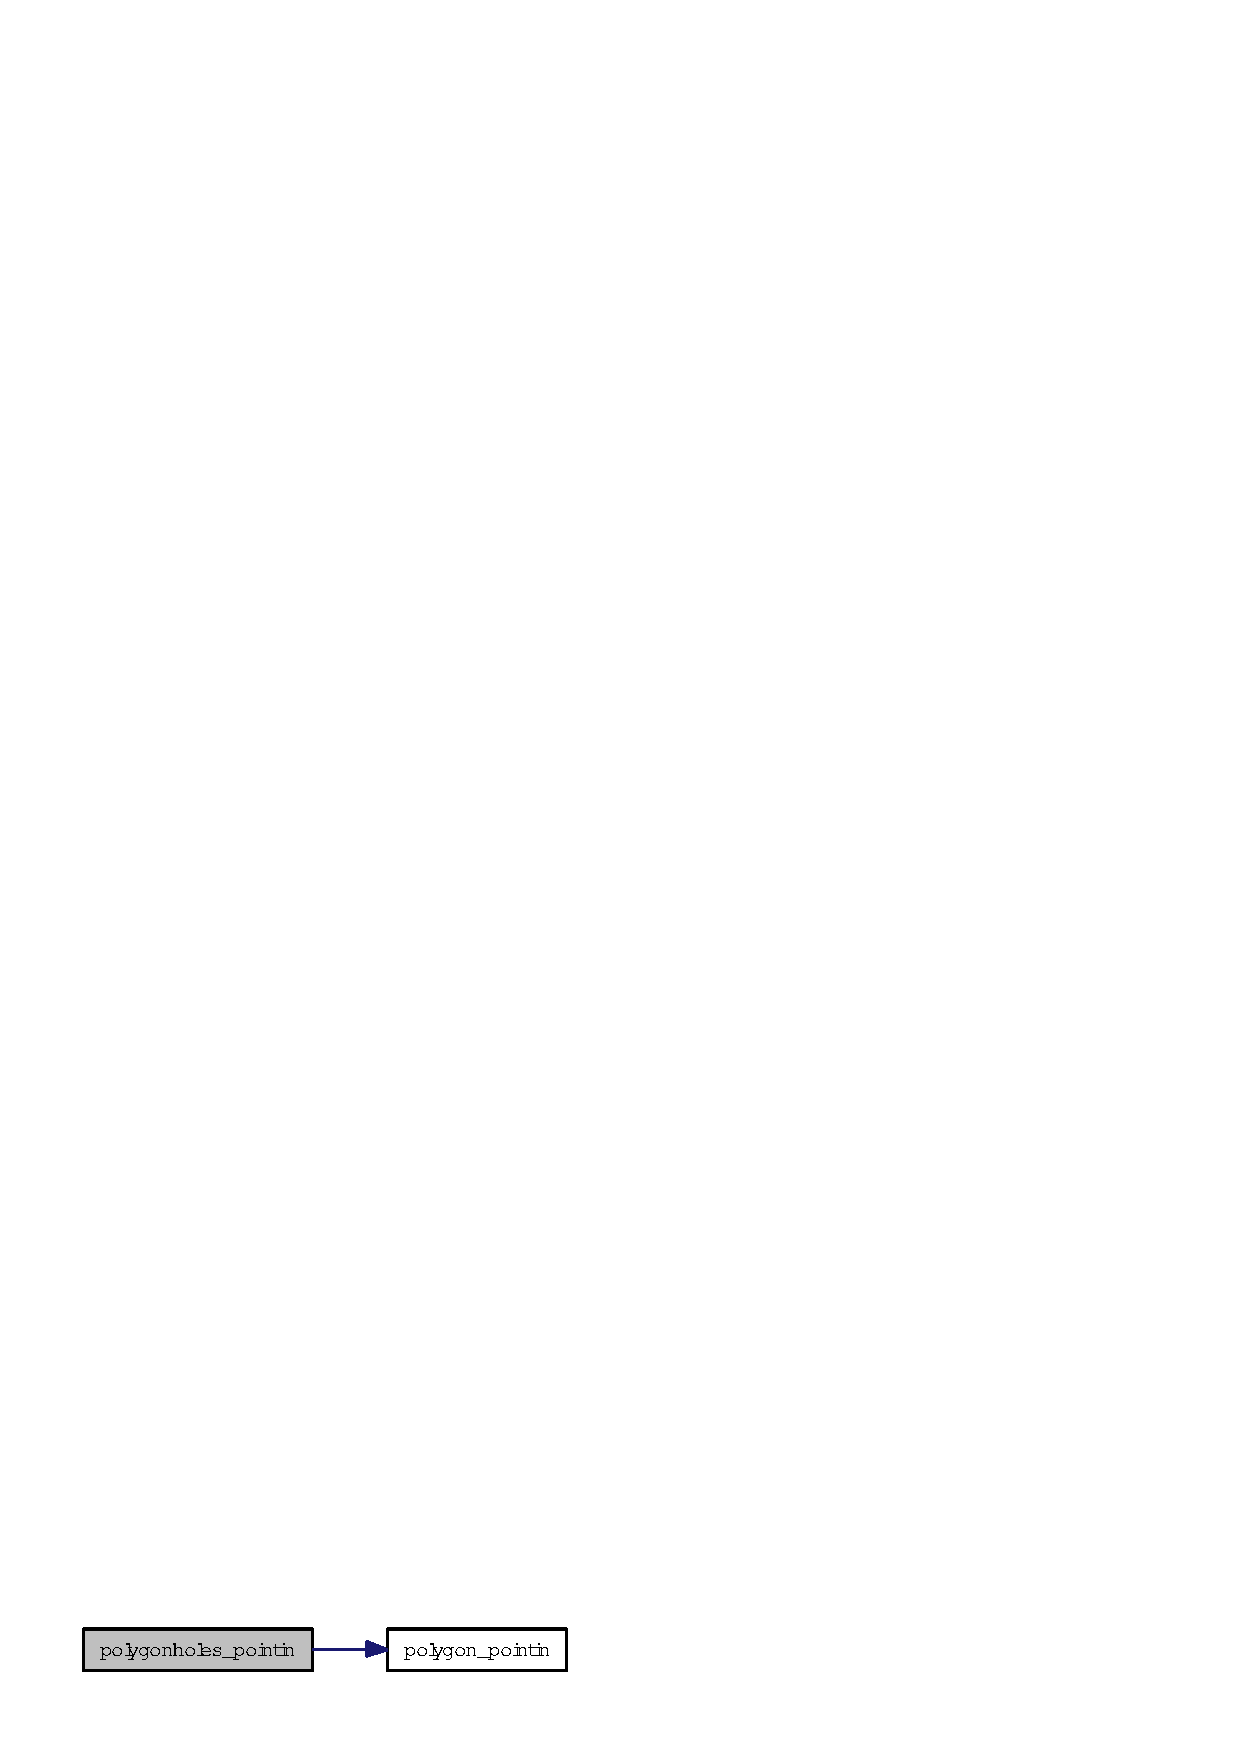
\includegraphics[width=138pt]{group__geometry_g35a6dd45f6d0cbed26ef8a69ed34a2e9_g35a6dd45f6d0cbed26ef8a69ed34a2e9_cgraph}
\end{center}
\end{figure}


Here is the caller graph for this function:\begin{figure}[H]
\begin{center}
\leavevmode
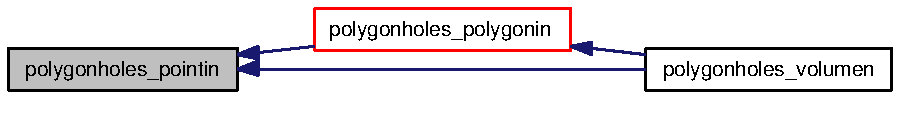
\includegraphics[width=234pt]{group__geometry_g35a6dd45f6d0cbed26ef8a69ed34a2e9_g35a6dd45f6d0cbed26ef8a69ed34a2e9_icgraph}
\end{center}
\end{figure}
\hypertarget{group__geometry_g139317720b027c782db9424256ba2c2d_g139317720b027c782db9424256ba2c2d}{
\index{geometry@{geometry}!polygonholes_pointinhole@{polygonholes\_\-pointinhole}}
\index{polygonholes_pointinhole@{polygonholes\_\-pointinhole}!geometry@{geometry}}
\subsubsection[polygonholes\_\-pointinhole]{\setlength{\rightskip}{0pt plus 5cm}bool polygonholes\_\-pointinhole (\hyperlink{struct__polygon__holes}{polygon\_\-holes} $\ast$ {\em p}, \hyperlink{struct__point}{point} $\ast$ {\em f})}}
\label{group__geometry_g139317720b027c782db9424256ba2c2d_g139317720b027c782db9424256ba2c2d}


Identifica si un punto esta dentro de un hueco del poligono.

\begin{Desc}
\item[Par\'{a}metros:]
\begin{description}
\item[\mbox{$\leftarrow$} {\em p}]Poligono Simple con huecos \item[\mbox{$\leftarrow$} {\em f}]Punto en 2 dimensiones \end{description}
\end{Desc}
\begin{Desc}
\item[Devuelve:]Verdadero si el punto esta dentro de uno de los huecos, falso en caso contrario \end{Desc}


Definici\'{o}n en la l\'{\i}nea 373 del archivo polygon\_\-holes.c.

\begin{Code}\begin{verbatim}374 {
375     bool valido=false;
376     unsigned int i;
377 
378     for (i=0;i<p->nholes && !valido;i++)
379     {
380         if (polygon_pointin(&(p->h[i]), f))
381         {
382             valido=true;
383         }
384     }
385     return valido;
386 }
\end{verbatim}\end{Code}




Gr\'{a}fico de llamadas para esta funci\'{o}n:\begin{figure}[H]
\begin{center}
\leavevmode
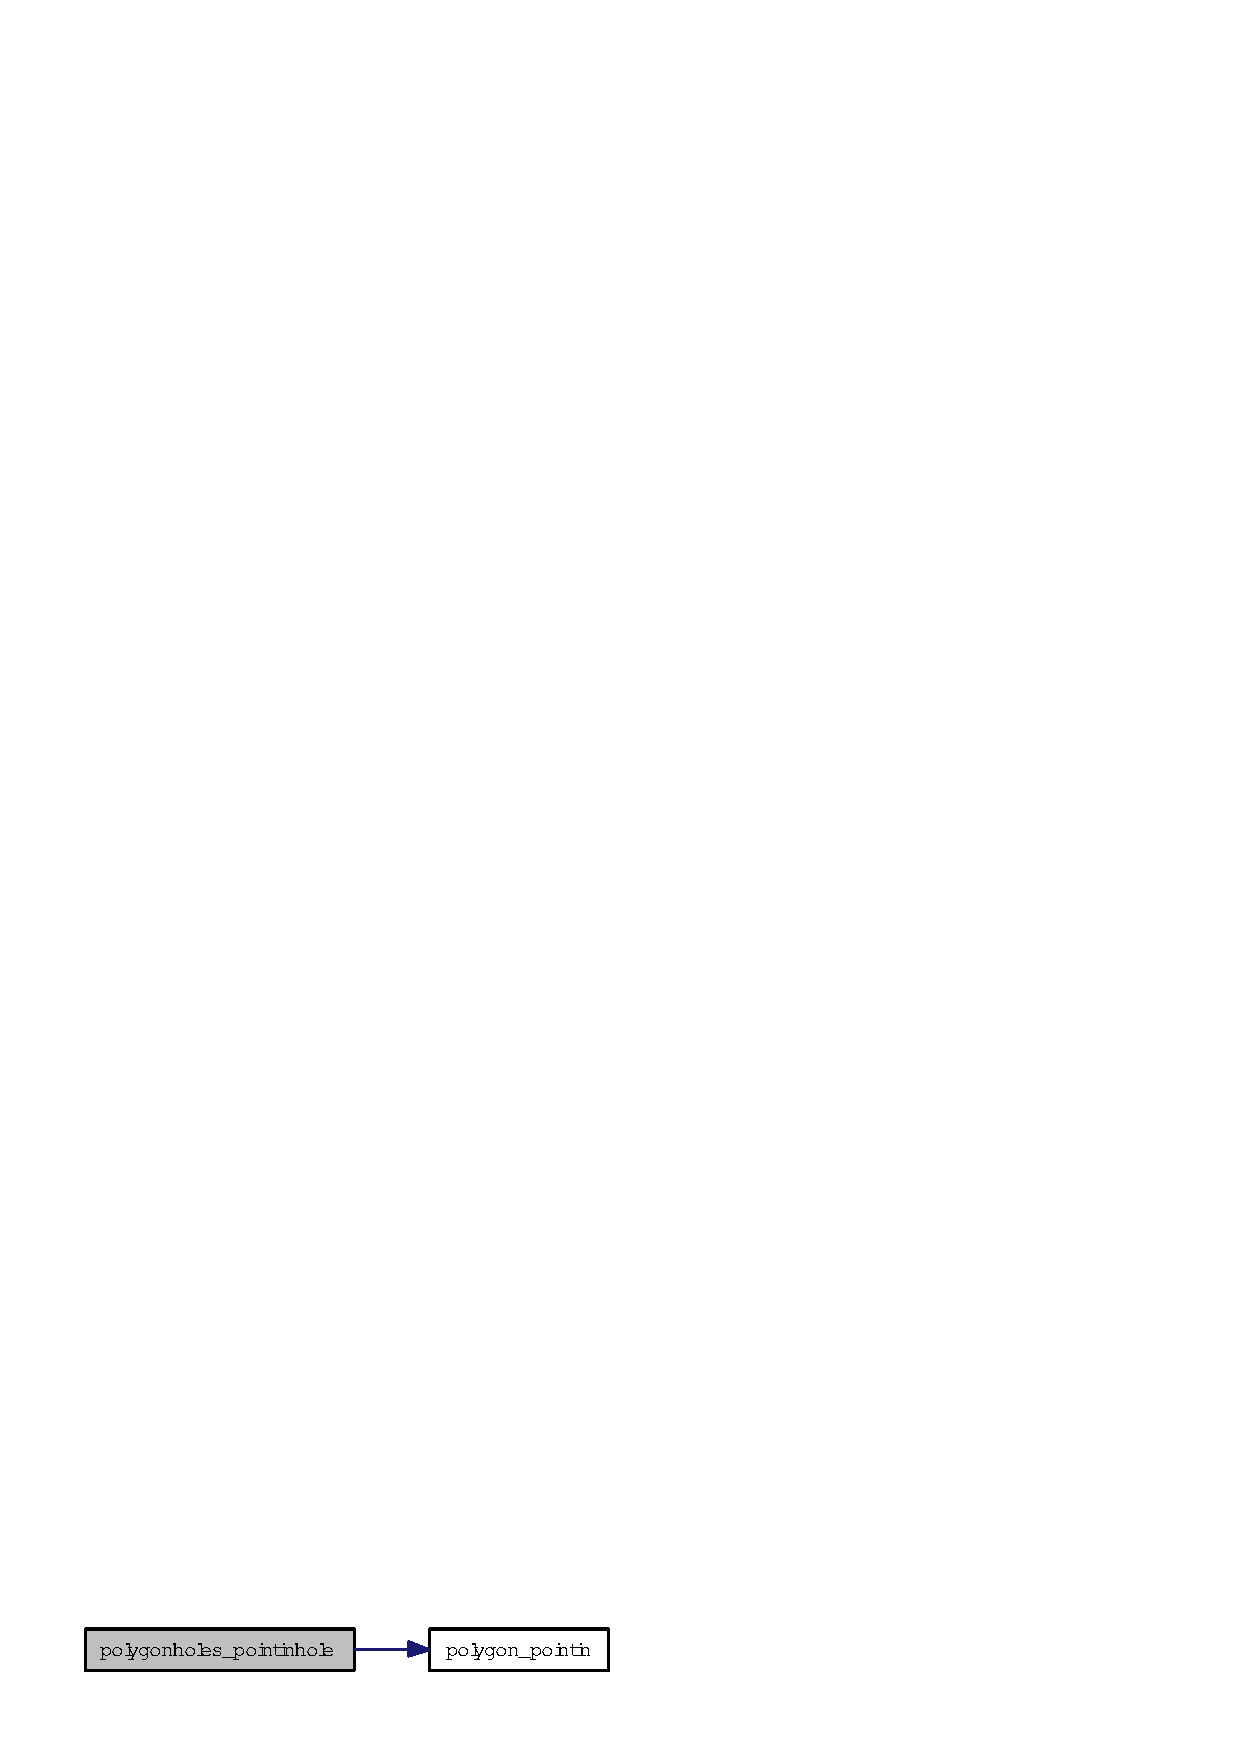
\includegraphics[width=148pt]{group__geometry_g139317720b027c782db9424256ba2c2d_g139317720b027c782db9424256ba2c2d_cgraph}
\end{center}
\end{figure}


Here is the caller graph for this function:\begin{figure}[H]
\begin{center}
\leavevmode
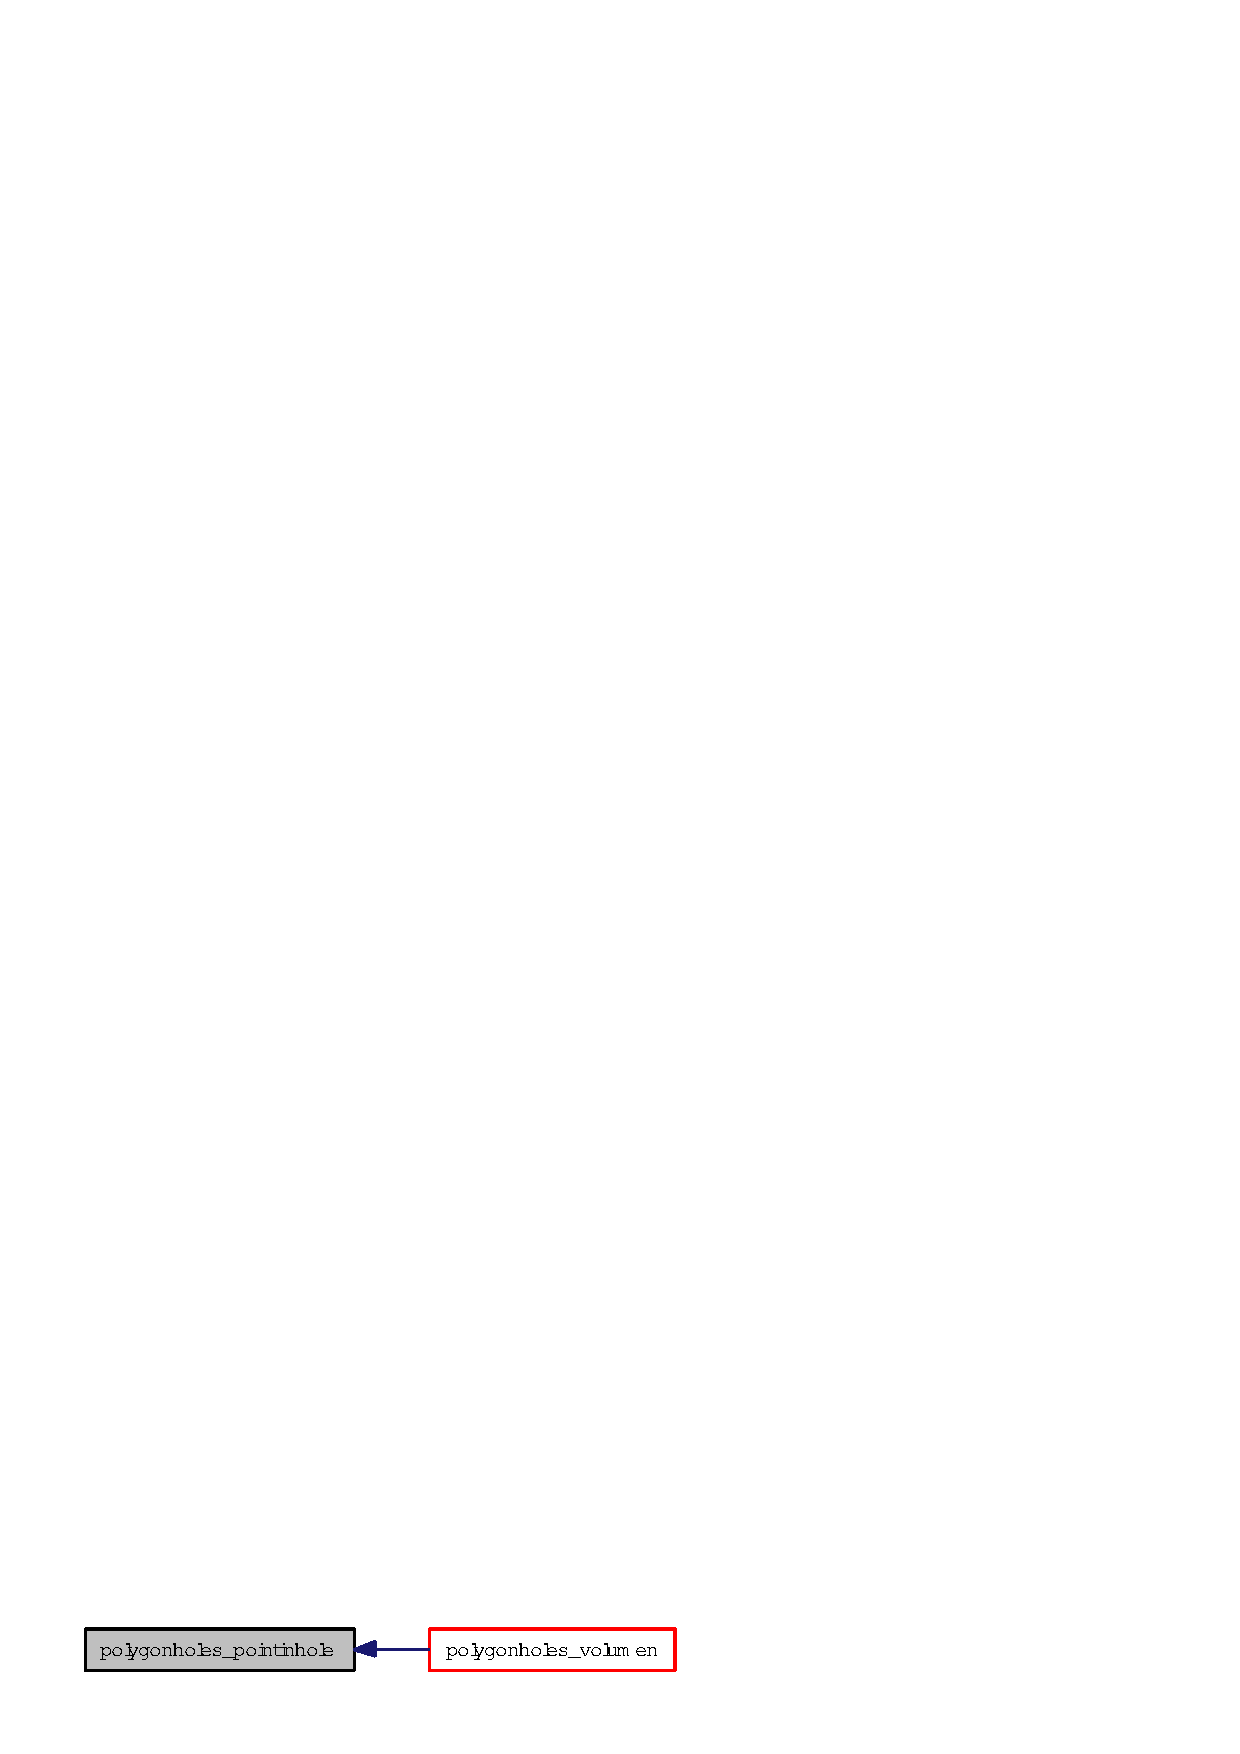
\includegraphics[width=164pt]{group__geometry_g139317720b027c782db9424256ba2c2d_g139317720b027c782db9424256ba2c2d_icgraph}
\end{center}
\end{figure}
\hypertarget{group__geometry_g496bae87588cb5710ced80f713da98ad_g496bae87588cb5710ced80f713da98ad}{
\index{geometry@{geometry}!polygonholes_polygonin@{polygonholes\_\-polygonin}}
\index{polygonholes_polygonin@{polygonholes\_\-polygonin}!geometry@{geometry}}
\subsubsection[polygonholes\_\-polygonin]{\setlength{\rightskip}{0pt plus 5cm}bool polygonholes\_\-polygonin (\hyperlink{struct__polygon__holes}{polygon\_\-holes} $\ast$ {\em p}, \hyperlink{struct__polygon}{polygon} $\ast$ {\em q})}}
\label{group__geometry_g496bae87588cb5710ced80f713da98ad_g496bae87588cb5710ced80f713da98ad}


La funcion evalua que el poligono q esta completamente adentro del poligono p entonces todos los puntos de q deben estar dentro de p y no se deben intersectar las lineas que los conforman

\begin{Desc}
\item[Par\'{a}metros:]
\begin{description}
\item[\mbox{$\leftarrow$} {\em p}]Poligono Simple con huecos \item[\mbox{$\leftarrow$} {\em q}]Poligono Simple \end{description}
\end{Desc}
\begin{Desc}
\item[Devuelve:]Verdadero en caso del que poligono q este dentro del poligono p, falso en caso contrario \end{Desc}


Definici\'{o}n en la l\'{\i}nea 399 del archivo polygon\_\-holes.c.

\begin{Code}\begin{verbatim}400 {
401     int i,j,k;
402     bool adentro = true;
403 
404     for (i=0;i<q->nvertices && adentro;i++)
405     {
406         line t1,t2;
407         t1.v1=q->v[i];
408         t1.v2=q->v[(i+1)%(q->nvertices)];
409 
410         if (!polygonholes_pointin(p,&q->v[i]))
411             adentro = false;
412 
413         if (!polygonholes_pointin(p,&q->v[(i+1)%(q->nvertices)]))
414             adentro = false;
415 
416         for (j=0;j<p->p->nvertices && adentro;j++)
417         {
418             t2.v1=p->p->v[j];
419             t2.v2=p->p->v[(j+1)%p->p->nvertices];
420             if (line_intersection(&t1,&t2))
421                 adentro = false;
422         }
423 
424         for (j=0;j<p->nholes && adentro; j++)
425         {
426             for (k=0;k<p->h[j].nvertices && adentro; k++)
427             {
428                 t2.v1 = p->h[j].v[k];
429                 t2.v2 = p->h[j].v[(k+1)%p->h[j].nvertices];
430                 if (line_intersection(&t1,&t2))
431                     adentro = false;
432             }
433         }
434     }
435     return adentro;
436 }
\end{verbatim}\end{Code}




Gr\'{a}fico de llamadas para esta funci\'{o}n:\begin{figure}[H]
\begin{center}
\leavevmode
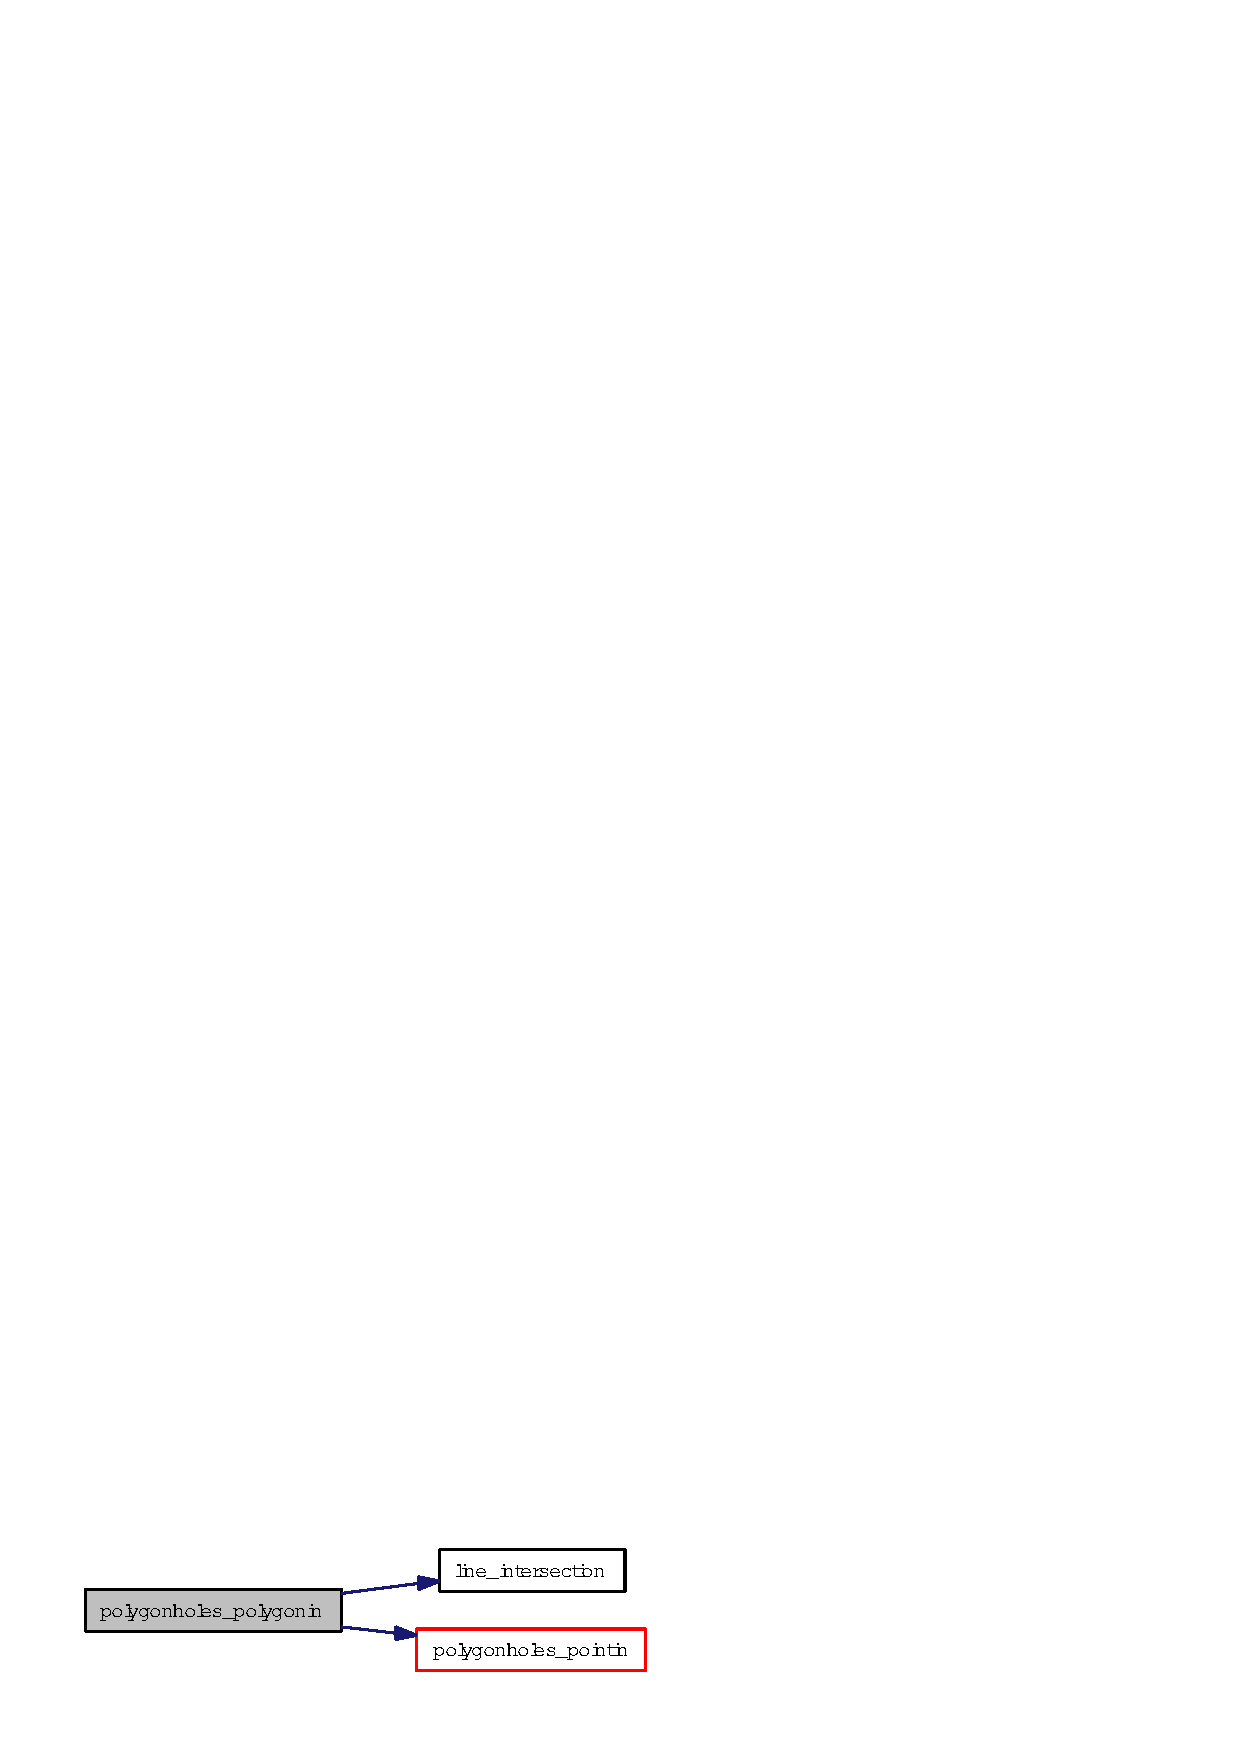
\includegraphics[width=157pt]{group__geometry_g496bae87588cb5710ced80f713da98ad_g496bae87588cb5710ced80f713da98ad_cgraph}
\end{center}
\end{figure}


Here is the caller graph for this function:\begin{figure}[H]
\begin{center}
\leavevmode
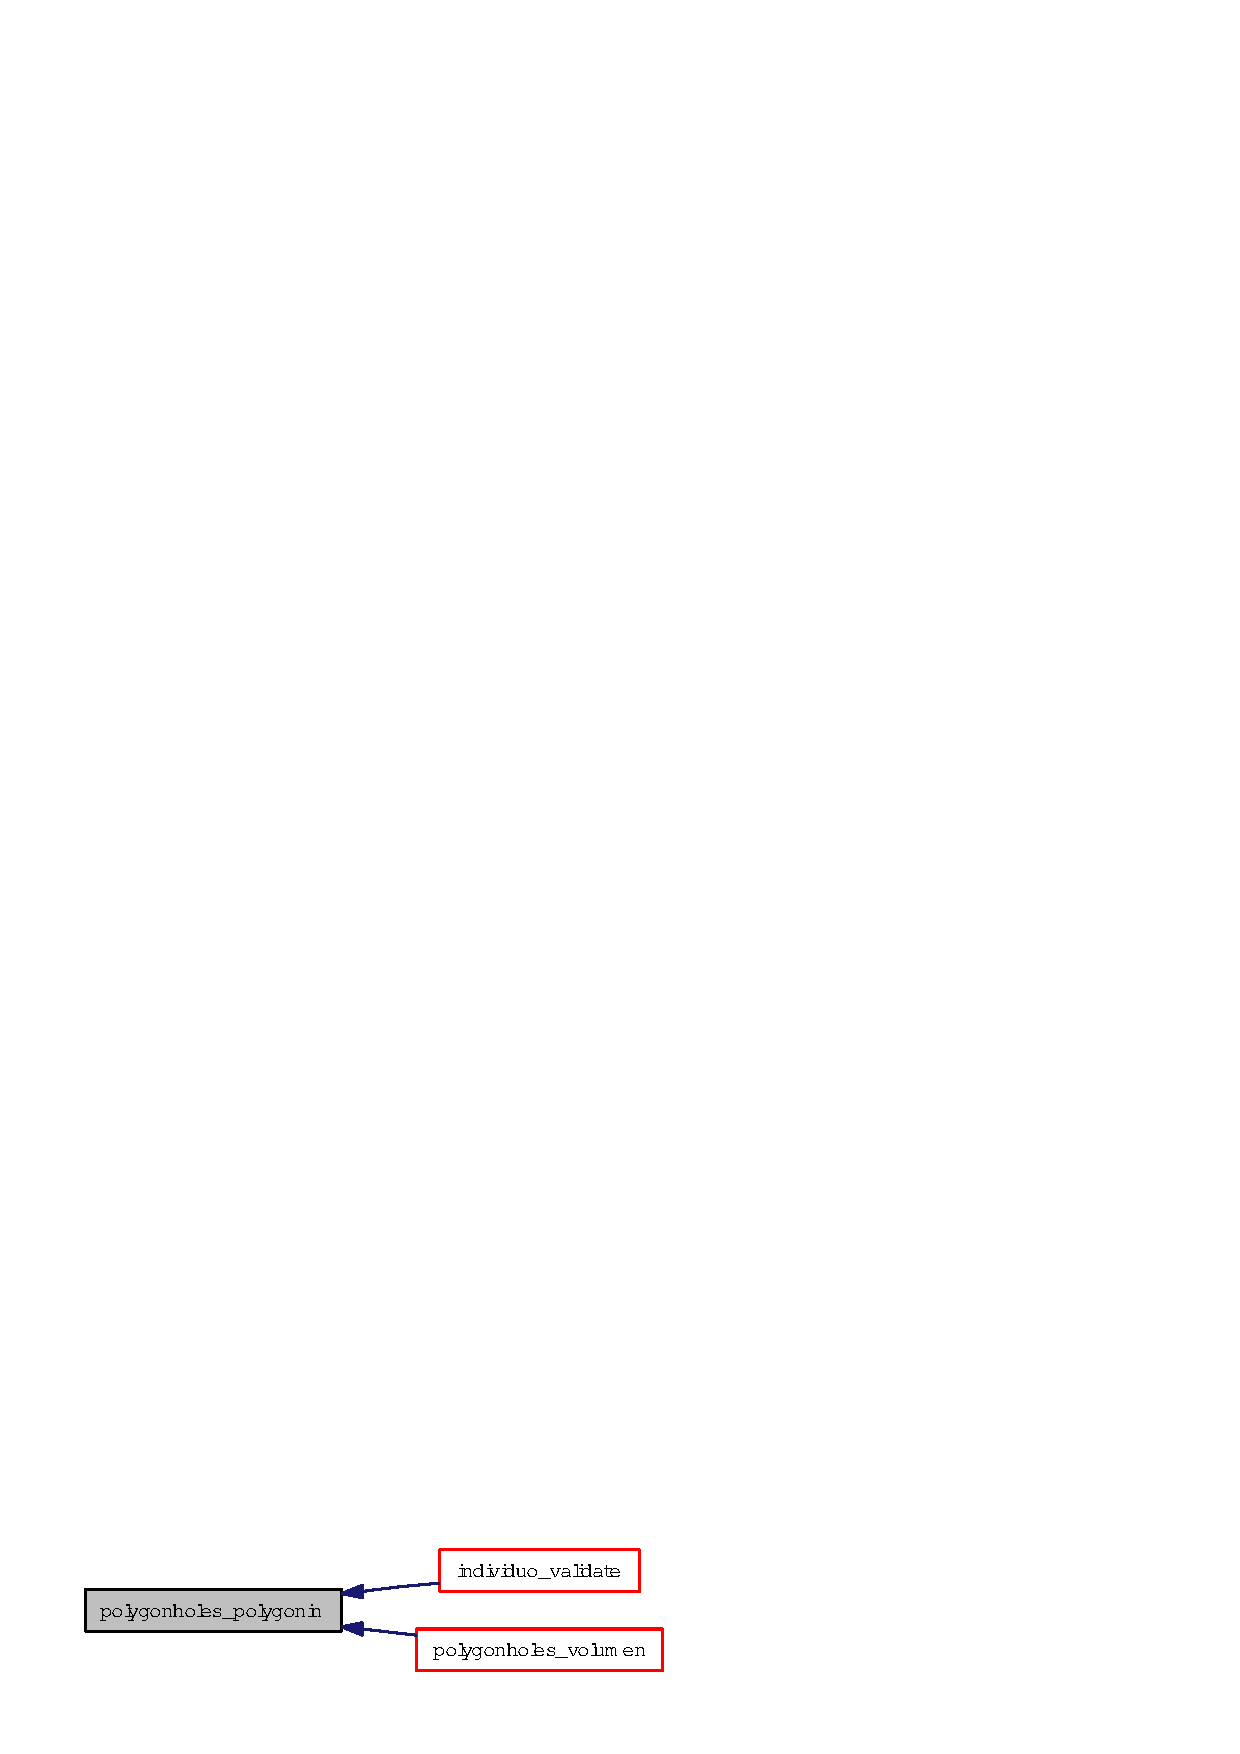
\includegraphics[width=161pt]{group__geometry_g496bae87588cb5710ced80f713da98ad_g496bae87588cb5710ced80f713da98ad_icgraph}
\end{center}
\end{figure}
\hypertarget{group__geometry_g7cf8b3f8c76179bb936754bbbf510999_g7cf8b3f8c76179bb936754bbbf510999}{
\index{geometry@{geometry}!polygonholes_volumen@{polygonholes\_\-volumen}}
\index{polygonholes_volumen@{polygonholes\_\-volumen}!geometry@{geometry}}
\subsubsection[polygonholes\_\-volumen]{\setlength{\rightskip}{0pt plus 5cm}float polygonholes\_\-volumen (\hyperlink{struct__polygon__holes}{polygon\_\-holes} $\ast$ {\em p})}}
\label{group__geometry_g7cf8b3f8c76179bb936754bbbf510999_g7cf8b3f8c76179bb936754bbbf510999}


Calcula el volumen generado por el poligono con huecos, definiendo asi el poligono como una figura tridimensional de la siguiente manera, la base del solido esta conformada por el poligono con huecos y la altura del solido en cada punto es igual a la distancia del punto a uno de los bordes.

El metodo para calcular el volumen se basa en encerrar el poligono en un rectangulo que lo contenga, y sucesivamente partir el poligono en dos subrectangulos respecto al lado mas largo calculando el volumen de cada uno de los subrectangulos y sumando el valor y esto se hace de manera recursiva.

\begin{itemize}
\item Cuando el subrectangulo esta completamente fuera del poligono no calculamos el volumen y regresamos un valor de 0\end{itemize}


\begin{itemize}
\item Cuando el subrectangulo tiene un area muy pequena definida por un da se calcula el centro del subrectangulo y se verifica que este dentro del poligono, si este es el caso, entonces se devuelve el valor del area multiplicada por la distancia del punto medio al borde, si el punto medio es 0 se devuelve 0.\end{itemize}


\begin{itemize}
\item Cuando el subrectangulo esta dentro del poligono y los vertices de este tienen su menor distancia respecto a un mismo segmento de recta se calcula el volumen del poliedro formado como el promedio de las distancias de los vertices multiplicados por el area del subrectangulo.\end{itemize}


\begin{itemize}
\item Cuando el subrectangulo esta dentro del poligono y los vertices de este tienen su menor distancia respecto a un mismo punto, que se da en el caso de los poligonos concavos, entonces se calcula el volumen como el volumen formado por la interseccion entre el cono que genera el punto y el subrectangulo, la formula que da este volumen es: $\int_{a}^{b}\int_{c}^{d}\sqrt{((x-h)^2 + (y-k)^2)} dx dy$ donde $(h,k)$ son las coordenadas del punto con respecto al que se toma la distancia, $(a,b)$ son los valores en que se desplaza $y$, $(c,d)$ son los valores en que se desplaza $x$.\end{itemize}


Esta funcion evalua menos puntos si en ves de dividir el rectangulo en 2 segun su lado mas largo, se divide en 4 partes iguales, pero esta aproximacion puede tener problemas cuando la proporcion del los lados del subrectangulo es muy grande.

\begin{Desc}
\item[Par\'{a}metros:]
\begin{description}
\item[\mbox{$\leftarrow$} {\em p}]Poligono simple con huecos en 2 dimensiones \end{description}
\end{Desc}
\begin{Desc}
\item[Devuelve:]Volumen generado \end{Desc}


\begin{Desc}
\item[\hyperlink{bug__bug000001}{Bug}]Esta funcion para calcular el volument de un rectangulo que intersecta un cono tiene valores indeterminados en algunos segmentos del problema, es posible que este error aparesca solo en algunos casos, pero hay que examinar mas la funcion. \end{Desc}


Definici\'{o}n en la l\'{\i}nea 86 del archivo polygon\_\-holes.c.

\begin{Code}\begin{verbatim}87 {
88 #if graphics
89     void draw_polygon(polygon *p)
90     {
91         int i;
92         for (i=0;i<p->nvertices;i++)
93         {
94             draw_line(p->v[i].x,p->v[i].y,p->v[(i+1)%p->nvertices].x,p->v[(i+1)%p->nvertices].y);
95         }
96     }
97 #endif
98 
99     float polygonholes_volumen_box( polygon_holes *p,
100                                     float minx,
101                                     float miny,
102                                     float maxx,
103                                     float maxy)
104     {
105 
106         float vol=0;
107         float da;
108 
109         polygon rec;
110         point q[4];
111 
112         q[0].x = minx;
113         q[0].y = miny;
114 
115         q[1].x = maxx;
116         q[1].y = miny;
117 
118         q[2].x = maxx;
119         q[2].y = maxy;
120 
121         q[3].x = minx;
122         q[3].y = maxy;
123 
124         rec.v =(point *) &q;
125         rec.nvertices = 4;
126 
127         da = polygon_area(&rec);
128 
129 
130         if (!polygon_overlapping(p->p, &rec)) //OK
131         {
132             vol = 0;
133 #if graphics
134 
135             draw_rect(minx, miny, maxx, maxy,255,255,255);
136 #endif
137 
138         }
139         else if (da < DELTA) // OK
140         {
141             point pm;
142 
143             pm.x=minx+((maxx-minx)/2.0);
144             pm.y=miny+((maxy-miny)/2.0);
145 
146             if (polygonholes_pointin(p, &pm))
147             {
148                 vol = da * distance_pointpolygonholes(&pm, p,NULL);
149 #if graphics
150 
151                 draw_rect(minx, miny, maxx, maxy,128,128,128);
152 #endif
153 
154             }
155             else
156             {
157                 vol = 0;
158 #if graphics
159 
160                 draw_rect(minx, miny, maxx, maxy,225,255,255);
161 #endif
162 
163             }
164         }
165         else
166         {
167 
168             int i;
169             float dis[4];
170             line ref[4];
171             for (i=0;i<4;i++)
172             {
173                 dis[i]=distance_pointpolygonholes(&q[i], p,&ref[i]);
174             }
175 
176             if( polygonholes_polygonin(p, &rec)
177                     &&
178                     (line_equal(&ref[0],&ref[1]) &&
179                      line_equal(&ref[1],&ref[2]) &&
180                      line_equal(&ref[2],&ref[3]))
181 
182               ) // OK
183             {
184                 if (line_ispoint(&ref[0]))// Si es un punto entonces se utiliza la formula del cono
185                 {
186                     double a,b,c,d,h,k;
187                     c=minx;
188                     d=maxx;
189                     a=miny;
190                     b=maxy;
191                     h=ref[0].v1.x;
192                     k=ref[0].v1.y;
193                     /*!\bug
194                     Esta funcion para calcular el volument de un rectangulo que intersecta un
195                     cono tiene valores indeterminados en algunos segmentos del problema, es
196                     posible que este error aparesca solo en algunos casos, pero hay que examinar
197                     mas la funcion.
198                     */
199 
200                     vol = (2*a*c*sqrt(pow(-c + h,2) + pow(a - k,2))
201                            - 2*a*h*sqrt(pow(-c + h,2) + pow(a - k,2))
202                            - 2*a*d*sqrt(pow(-d + h,2) + pow(a - k,2))
203                            + 2*a*h*sqrt(pow(-d + h,2) + pow(a - k,2))
204                            - 2*b*c*sqrt(pow(-c + h,2) + pow(b - k,2))
205                            + 2*b*h*sqrt(pow(-c + h,2) + pow(b - k,2))
206                            + 2*b*d*sqrt(pow(-d + h,2) + pow(b - k,2))
207                            - 2*b*h*sqrt(pow(-d + h,2) + pow(b - k,2))
208                            - 2*c*k*sqrt(pow(-c + h,2) + pow(a - k,2))
209                            + 2*h*k*sqrt(pow(-c + h,2) + pow(a - k,2))
210                            + 2*d*k*sqrt(pow(-d + h,2) + pow(a - k,2))
211                            - 2*h*k*sqrt(pow(-d + h,2) + pow(a - k,2))
212                            + 2*c*k*sqrt(pow(-c + h,2) + pow(b - k,2))
213                            - 2*h*k*sqrt(pow(-c + h,2) + pow(b - k,2))
214                            - 2*d*k*sqrt(pow(-d + h,2) + pow(b - k,2))
215                            + 2*h*k*sqrt(pow(-d + h,2) + pow(b - k,2))
216                            - pow(a,3)*log(-c + h + sqrt(pow(-c + h,2) + pow(a - k,2)))
217                            + 3*pow(a,2)*k*log(-c + h + sqrt(pow(-c + h,2) + pow(a - k,2)))
218                            - 3*a*pow(k,2)*log(-c + h + sqrt(pow(-c + h,2) + pow(a - k,2)))
219                            + pow(k,3)*log(-c + h + sqrt(pow(-c + h,2) + pow(a - k,2)))
220                            + pow(a,3)*log(-d + h + sqrt(pow(-d + h,2) + pow(a - k,2)))
221                            - 3*pow(a,2)*k*log(-d + h + sqrt(pow(-d + h,2) + pow(a - k,2)))
222                            + 3*a*pow(k,2)*log(-d + h + sqrt(pow(-d + h,2) + pow(a - k,2)))
223                            - pow(k,3)*log(-d + h + sqrt(pow(-d + h,2) + pow(a - k,2)))
224                            + pow(b,3)*log(-c + h + sqrt(pow(-c + h,2) + pow(b - k,2)))
225                            - 3*pow(b,2)*k*log(-c + h + sqrt(pow(-c + h,2) + pow(b - k,2)))
226                            + 3*b*pow(k,2)*log(-c + h + sqrt(pow(-c + h,2) + pow(b - k,2)))
227                            - pow(k,3)*log(-c + h + sqrt(pow(-c + h,2) + pow(b - k,2)))
228                            - pow(b,3)*log(-d + h + sqrt(pow(-d + h,2) + pow(b - k,2)))
229                            + 3*pow(b,2)*k*log(-d + h + sqrt(pow(-d + h,2) + pow(b - k,2)))
230                            - 3*b*pow(k,2)*log(-d + h + sqrt(pow(-d + h,2) + pow(b - k,2)))
231                            + pow(k,3)*log(-d + h + sqrt(pow(-d + h,2) + pow(b - k,2)))
232                            + pow(c,3)*log(a + sqrt(pow(-c + h,2) + pow(a - k,2)) - k)
233                            - 3*pow(c,2)*h*log(a + sqrt(pow(-c + h,2) + pow(a - k,2)) - k)
234                            + 3*c*pow(h,2)*log(a + sqrt(pow(-c + h,2) + pow(a - k,2)) - k)
235                            - pow(h,3)*log(a + sqrt(pow(-c + h,2) + pow(a - k,2)) - k)
236                            - pow(d,3)*log(a + sqrt(pow(-d + h,2) + pow(a - k,2)) - k)
237                            + 3*pow(d,2)*h*log(a + sqrt(pow(-d + h,2) + pow(a - k,2)) - k)
238                            - 3*d*pow(h,2)*log(a + sqrt(pow(-d + h,2) + pow(a - k,2)) - k)
239                            + pow(h,3)*log(a + sqrt(pow(-d + h,2) + pow(a - k,2)) - k)
240                            - pow(c,3)*log(b + sqrt(pow(-c + h,2) + pow(b - k,2)) - k)
241                            + 3*pow(c,2)*h*log(b + sqrt(pow(-c + h,2) + pow(b - k,2)) - k)
242                            - 3*c*pow(h,2)*log(b + sqrt(pow(-c + h,2) + pow(b - k,2)) - k)
243                            + pow(h,3)*log(b + sqrt(pow(-c + h,2) + pow(b - k,2)) - k)
244                            + pow(d,3)*log(b + sqrt(pow(-d + h,2) + pow(b - k,2)) - k)
245                            - 3*pow(d,2)*h*log(b + sqrt(pow(-d + h,2) + pow(b - k,2)) - k)
246                            + 3*d*pow(h,2)*log(b + sqrt(pow(-d + h,2) + pow(b - k,2)) - k)
247                            - pow(h,3)*log(b + sqrt(pow(-d + h,2) + pow(b - k,2)) - k))/6;
248 #if graphics
249 
250                     draw_rect(minx, miny, maxx, maxy,0,128,0);
251 #endif
252 
253                 }
254                 else // Si es una linea se utiliza la formula de la cuna
255                 {
256                     vol = (dis[0]+dis[1]+dis[2]+dis[3])/4.0 * da;
257 #if graphics
258 
259                     draw_rect(minx, miny, maxx, maxy,0,0,128);
260 #endif
261 
262                 }
263             }
264             else
265             {
266                 if (!(
267                             polygonholes_pointinhole(p, &q[0]) &&
268                             polygonholes_pointinhole(p, &q[1]) &&
269                             polygonholes_pointinhole(p, &q[2]) &&
270                             polygonholes_pointinhole(p, &q[3])
271                         )) // el poligono esta dentro de p pero no en un hueco
272                 {
273                     //Opcion de corte 1
274                     /*
275                                         vol+= polygonholes_volumen_box(p, minx, miny, (minx+maxx)/2.0, (miny+maxy)/2.0);
276                                         vol+= polygonholes_volumen_box(p, (minx+maxx)/2.0, miny, maxx, (miny+maxy)/2.0);
277                                         vol+= polygonholes_volumen_box(p, minx, (miny+maxy)/2.0, (minx+maxx)/2.0, maxy);
278                                         vol+= polygonholes_volumen_box(p, (minx+maxx)/2.0, (miny+maxy)/2.0, maxx, maxy);
279                     */
280 
281                     if (maxx-minx > maxy-miny)
282                     {
283                         vol+= polygonholes_volumen_box(p, minx, miny, (minx+maxx)/2.0, maxy);
284                         vol+= polygonholes_volumen_box(p, (minx+maxx)/2.0, miny, maxx, maxy);
285                     }
286                     else
287                     {
288                         vol+= polygonholes_volumen_box(p, minx, miny, maxx, (miny+maxy)/2.0);
289                         vol+= polygonholes_volumen_box(p, minx, (miny+maxy)/2.0, maxx, maxy);
290                     }
291 
292                 }
293 #if graphics
294                 else
295                 {
296                     draw_rect(minx, miny, maxx, maxy,0,0,255);
297                 }
298 #endif
299 
300             }
301         }
302         if (isnan(vol))
303         {
304 #if graphics
305             draw_rect(minx, miny, maxx, maxy,255,0,0);
306 #endif
307 
308             fprintf(stderr,"Error: (%f, %f) (%f, %f)\n",minx,miny,maxx,maxy);
309             vol=0;
310         }
311         return vol;
312     }
313 
314     float minx, miny, maxx, maxy;
315     polygon_minbox(p->p, &minx, &miny, &maxx, &maxy);
316 
317 #if graphics
318     getscreen();
319     clearscreen();
320     draw_polygon(p->p);
321 
322     {
323         int j;
324         for (j=0;j<p->nholes;j++)
325         {
326             draw_polygon(&(p->h[j]));
327         }
328     }
329     relscreen();
330 #endif
331 
332     return polygonholes_volumen_box(p,minx,miny,maxx,maxy);
333 }
\end{verbatim}\end{Code}




Gr\'{a}fico de llamadas para esta funci\'{o}n:\begin{figure}[H]
\begin{center}
\leavevmode
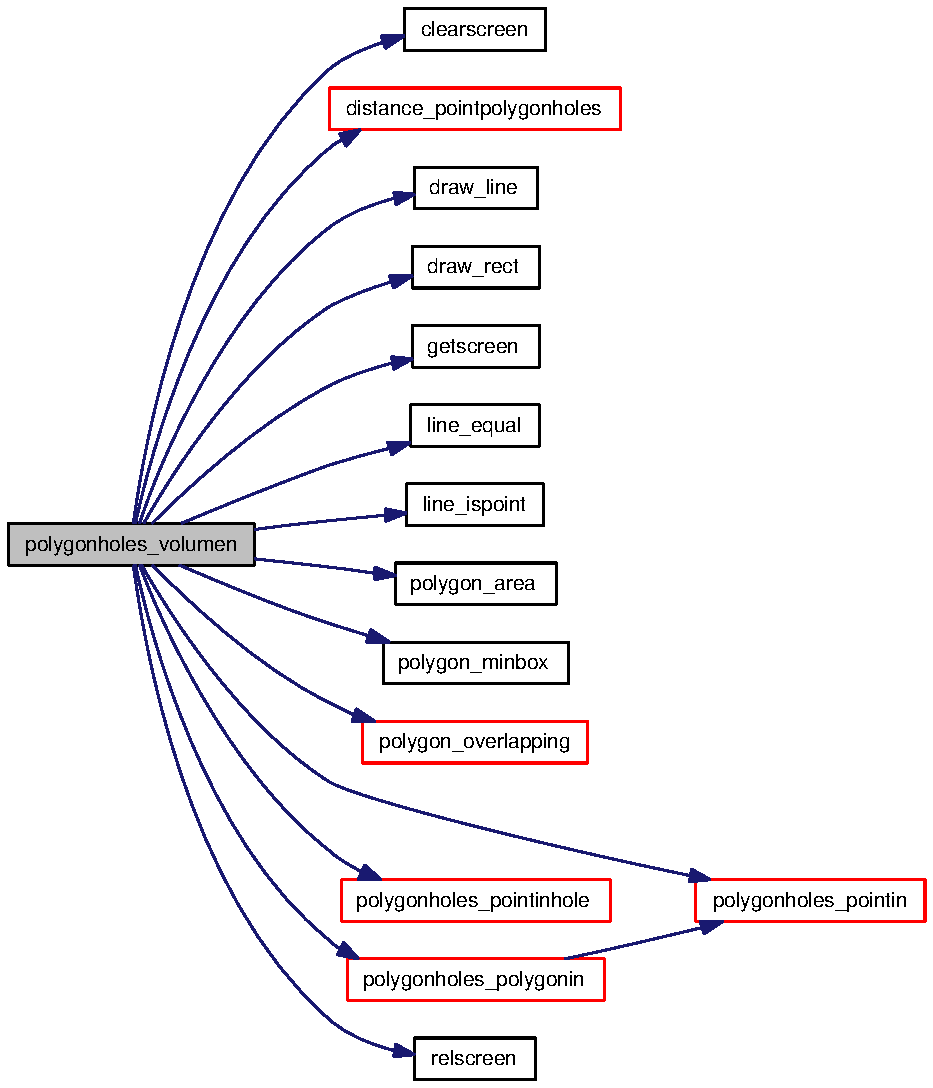
\includegraphics[width=242pt]{group__geometry_g7cf8b3f8c76179bb936754bbbf510999_g7cf8b3f8c76179bb936754bbbf510999_cgraph}
\end{center}
\end{figure}


Here is the caller graph for this function:\begin{figure}[H]
\begin{center}
\leavevmode
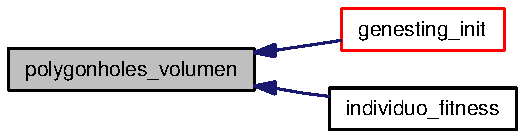
\includegraphics[width=144pt]{group__geometry_g7cf8b3f8c76179bb936754bbbf510999_g7cf8b3f8c76179bb936754bbbf510999_icgraph}
\end{center}
\end{figure}
